% Options for packages loaded elsewhere
% Options for packages loaded elsewhere
\PassOptionsToPackage{unicode}{hyperref}
\PassOptionsToPackage{hyphens}{url}
\PassOptionsToPackage{dvipsnames,svgnames,x11names}{xcolor}
%
\documentclass[
  12pt,
]{article}
\usepackage{xcolor}
\usepackage[margin=2.5cm]{geometry}
\usepackage{amsmath,amssymb}
\setcounter{secnumdepth}{-\maxdimen} % remove section numbering
\usepackage{iftex}
\ifPDFTeX
  \usepackage[T1]{fontenc}
  \usepackage[utf8]{inputenc}
  \usepackage{textcomp} % provide euro and other symbols
\else % if luatex or xetex
  \usepackage{unicode-math} % this also loads fontspec
  \defaultfontfeatures{Scale=MatchLowercase}
  \defaultfontfeatures[\rmfamily]{Ligatures=TeX,Scale=1}
\fi
\usepackage{lmodern}
\ifPDFTeX\else
  % xetex/luatex font selection
\fi
% Use upquote if available, for straight quotes in verbatim environments
\IfFileExists{upquote.sty}{\usepackage{upquote}}{}
\IfFileExists{microtype.sty}{% use microtype if available
  \usepackage[]{microtype}
  \UseMicrotypeSet[protrusion]{basicmath} % disable protrusion for tt fonts
}{}
\makeatletter
\@ifundefined{KOMAClassName}{% if non-KOMA class
  \IfFileExists{parskip.sty}{%
    \usepackage{parskip}
  }{% else
    \setlength{\parindent}{0pt}
    \setlength{\parskip}{6pt plus 2pt minus 1pt}}
}{% if KOMA class
  \KOMAoptions{parskip=half}}
\makeatother
% Make \paragraph and \subparagraph free-standing
\makeatletter
\ifx\paragraph\undefined\else
  \let\oldparagraph\paragraph
  \renewcommand{\paragraph}{
    \@ifstar
      \xxxParagraphStar
      \xxxParagraphNoStar
  }
  \newcommand{\xxxParagraphStar}[1]{\oldparagraph*{#1}\mbox{}}
  \newcommand{\xxxParagraphNoStar}[1]{\oldparagraph{#1}\mbox{}}
\fi
\ifx\subparagraph\undefined\else
  \let\oldsubparagraph\subparagraph
  \renewcommand{\subparagraph}{
    \@ifstar
      \xxxSubParagraphStar
      \xxxSubParagraphNoStar
  }
  \newcommand{\xxxSubParagraphStar}[1]{\oldsubparagraph*{#1}\mbox{}}
  \newcommand{\xxxSubParagraphNoStar}[1]{\oldsubparagraph{#1}\mbox{}}
\fi
\makeatother


\usepackage{longtable,booktabs,array}
\usepackage{calc} % for calculating minipage widths
% Correct order of tables after \paragraph or \subparagraph
\usepackage{etoolbox}
\makeatletter
\patchcmd\longtable{\par}{\if@noskipsec\mbox{}\fi\par}{}{}
\makeatother
% Allow footnotes in longtable head/foot
\IfFileExists{footnotehyper.sty}{\usepackage{footnotehyper}}{\usepackage{footnote}}
\makesavenoteenv{longtable}
\usepackage{graphicx}
\makeatletter
\newsavebox\pandoc@box
\newcommand*\pandocbounded[1]{% scales image to fit in text height/width
  \sbox\pandoc@box{#1}%
  \Gscale@div\@tempa{\textheight}{\dimexpr\ht\pandoc@box+\dp\pandoc@box\relax}%
  \Gscale@div\@tempb{\linewidth}{\wd\pandoc@box}%
  \ifdim\@tempb\p@<\@tempa\p@\let\@tempa\@tempb\fi% select the smaller of both
  \ifdim\@tempa\p@<\p@\scalebox{\@tempa}{\usebox\pandoc@box}%
  \else\usebox{\pandoc@box}%
  \fi%
}
% Set default figure placement to htbp
\def\fps@figure{htbp}
\makeatother


% definitions for citeproc citations
\NewDocumentCommand\citeproctext{}{}
\NewDocumentCommand\citeproc{mm}{%
  \begingroup\def\citeproctext{#2}\cite{#1}\endgroup}
\makeatletter
 % allow citations to break across lines
 \let\@cite@ofmt\@firstofone
 % avoid brackets around text for \cite:
 \def\@biblabel#1{}
 \def\@cite#1#2{{#1\if@tempswa , #2\fi}}
\makeatother
\newlength{\cslhangindent}
\setlength{\cslhangindent}{1.5em}
\newlength{\csllabelwidth}
\setlength{\csllabelwidth}{3em}
\newenvironment{CSLReferences}[2] % #1 hanging-indent, #2 entry-spacing
 {\begin{list}{}{%
  \setlength{\itemindent}{0pt}
  \setlength{\leftmargin}{0pt}
  \setlength{\parsep}{0pt}
  % turn on hanging indent if param 1 is 1
  \ifodd #1
   \setlength{\leftmargin}{\cslhangindent}
   \setlength{\itemindent}{-1\cslhangindent}
  \fi
  % set entry spacing
  \setlength{\itemsep}{#2\baselineskip}}}
 {\end{list}}
\usepackage{calc}
\newcommand{\CSLBlock}[1]{\hfill\break\parbox[t]{\linewidth}{\strut\ignorespaces#1\strut}}
\newcommand{\CSLLeftMargin}[1]{\parbox[t]{\csllabelwidth}{\strut#1\strut}}
\newcommand{\CSLRightInline}[1]{\parbox[t]{\linewidth - \csllabelwidth}{\strut#1\strut}}
\newcommand{\CSLIndent}[1]{\hspace{\cslhangindent}#1}



\setlength{\emergencystretch}{3em} % prevent overfull lines

\providecommand{\tightlist}{%
  \setlength{\itemsep}{0pt}\setlength{\parskip}{0pt}}



 


\makeatletter
\@ifpackageloaded{caption}{}{\usepackage{caption}}
\AtBeginDocument{%
\ifdefined\contentsname
  \renewcommand*\contentsname{Table of contents}
\else
  \newcommand\contentsname{Table of contents}
\fi
\ifdefined\listfigurename
  \renewcommand*\listfigurename{List of Figures}
\else
  \newcommand\listfigurename{List of Figures}
\fi
\ifdefined\listtablename
  \renewcommand*\listtablename{List of Tables}
\else
  \newcommand\listtablename{List of Tables}
\fi
\ifdefined\figurename
  \renewcommand*\figurename{Figure}
\else
  \newcommand\figurename{Figure}
\fi
\ifdefined\tablename
  \renewcommand*\tablename{Table}
\else
  \newcommand\tablename{Table}
\fi
}
\@ifpackageloaded{float}{}{\usepackage{float}}
\floatstyle{ruled}
\@ifundefined{c@chapter}{\newfloat{codelisting}{h}{lop}}{\newfloat{codelisting}{h}{lop}[chapter]}
\floatname{codelisting}{Listing}
\newcommand*\listoflistings{\listof{codelisting}{List of Listings}}
\makeatother
\makeatletter
\makeatother
\makeatletter
\@ifpackageloaded{caption}{}{\usepackage{caption}}
\@ifpackageloaded{subcaption}{}{\usepackage{subcaption}}
\makeatother
\usepackage{bookmark}
\IfFileExists{xurl.sty}{\usepackage{xurl}}{} % add URL line breaks if available
\urlstyle{same}
\hypersetup{
  pdftitle={LLM-Assisted ESG Disclosure Assessment for Taiwan Listed Companies},
  pdfauthor={Paper Lab},
  colorlinks=true,
  linkcolor={blue},
  filecolor={Maroon},
  citecolor={blue},
  urlcolor={Blue},
  pdfcreator={LaTeX via pandoc}}


\title{LLM-Assisted ESG Disclosure Assessment for Taiwan Listed
Companies}
\author{Paper Lab}
\date{2026-03-27}
\begin{document}
\maketitle


\textbf{Background:} ESG disclosure assessment has increasingly relied
on keyword counts, checklist rules, and proprietary ratings, yet these
approaches often fail to capture semantic completeness, specificity,
consistency, and decision-usefulness in narrative reports. Prior
research has shown that disclosure precision and readability are
strategic choices rather than simple term-frequency outcomes, while
recent work indicates that modern language models may support
finer-grained document understanding when carefully validated against
human benchmarks LI and ZHANG (\citeproc{ref-LI2015}{2015}) Berger et
al. (\citeproc{ref-Berger2021}{2021}) Tong et al.
(\citeproc{ref-Tong2022}{2022}) Bender et al.
(\citeproc{ref-Bender2021}{2021}).

\textbf{Problem:} Existing ESG measurement methods remain limited in
Chinese and bilingual reporting contexts, and weak validation against
expert judgment creates uncertainty about whether automated scores
reflect substantive disclosure quality. This limitation is especially
relevant for Taiwan-listed companies, where report language and
disclosure practices are heterogeneous and context dependent Zhao et al.
(\citeproc{ref-Zhao2021}{2021}) Wu et al. (\citeproc{ref-Wu2022}{2022})
Wang and Chen (\citeproc{ref-Wang2017}{2017}).

\textbf{Method:} This study proposes an LLM-assisted framework for ESG
disclosure assessment using annual and sustainability reports of
Taiwan-listed firms. Expert-coded benchmark ratings were constructed for
ESG disclosure quality, and LLM-generated scores were compared with
keyword-based and rule-based baselines. Agreement with human
evaluations, error metrics, and rank consistency were examined, and
firm-level regressions were estimated to explain variation in disclosure
quality.

\textbf{Results:} The LLM-assisted method aligned more closely with
expert ratings than conventional baselines and demonstrated stronger
performance across Environmental, Social, and Governance dimensions. The
method also differentiated disclosure quality more effectively across
firms and industries, with higher scores observed among firms with
stronger governance and greater foreign ownership.

\textbf{Conclusion:} The findings indicate that LLM-assisted semantic
evaluation offers a more accurate, scalable, and auditable approach to
ESG disclosure assessment than traditional text-counting methods, with
important implications for sustainability researchers, regulators,
investors, and reporting firms.

\section{Introduction}\label{introduction}

\subsection{Introduction}\label{introduction-1}

Environmental, social, and governance (ESG) disclosure has become an
increasingly salient mechanism through which listed firms communicate
sustainability-related risks, practices, and outcomes to capital market
participants, regulators, and other stakeholders. As ESG reporting has
expanded across jurisdictions, the quality of disclosure has emerged as
a central concern because decision-useful reporting must extend beyond
formal compliance to encompass completeness, specificity, consistency,
and relevance. Prior research on corporate narrative disclosure has
demonstrated that firms strategically vary disclosure precision and
readability in response to market incentives, indicating that the
informational content of reports cannot be inferred reliably from the
mere presence of topical terms alone LI and ZHANG
(\citeproc{ref-LI2015}{2015}). Complementary evidence from
sustainability and digital transformation research suggests that
disclosure quality is shaped by organizational capabilities, governance
structures, and strategic orientation, implying substantial
heterogeneity across firms and industries Gelhard and Delft
(\citeproc{ref-Gelhard2016}{2016}) Berger et al.
(\citeproc{ref-Berger2021}{2021}). In this context, ESG disclosure
assessment has become an important measurement problem, not merely a
descriptive accounting exercise.

Despite growing attention to ESG reporting, much of the existing
literature continues to rely on coarse proxies such as keyword counts,
checklist-based indices, or proprietary ESG ratings. Such approaches are
attractive because they can be implemented at scale, yet they often
treat disclosure as a frequency problem rather than a semantic one. In
practice, boilerplate language may be scored as informative, while
nuanced but less repetitive disclosures may be undervalued. This
limitation is especially consequential for sustainability reports, where
strategic ambiguity, repetition, and selective emphasis are common
features of corporate communication Park and Patel
(\citeproc{ref-Park2015}{2015}) LI and ZHANG
(\citeproc{ref-LI2015}{2015}). As a result, conventional disclosure
metrics may fail to distinguish between symbolic and substantive ESG
reporting, weakening both academic inference and practical benchmarking.

The need for improved measurement is particularly acute in Taiwan.
Taiwan-listed firms commonly publish annual reports and sustainability
reports in Chinese or bilingual formats, and disclosure practices vary
substantially across industries, ownership structures, and governance
environments. Existing studies in broader Asian settings indicate that
firms' sustainability-related communication and performance are
associated with capital market responses and organizational
characteristics Wang and Chen (\citeproc{ref-Wang2017}{2017}) Xianchuan
Yang, Jiang, and Chen (\citeproc{ref-Yang2022}{2022}). However,
comparatively little evidence has been developed on how ESG disclosure
quality itself should be measured in the Taiwan context. This gap
matters because multilingual reporting introduces additional complexity
for textual analysis, and translation or language-specific phrasing may
materially affect the interpretation of disclosure content Zhao et al.
(\citeproc{ref-Zhao2021}{2021}) Tong et al.
(\citeproc{ref-Tong2022}{2022}). Consequently, a context-sensitive and
linguistically robust method is required to evaluate disclosure quality
in a way that is both scalable and auditable.

Large language models (LLMs) provide a promising avenue for addressing
this measurement challenge. Recent advances in natural language
processing have shown that LLMs can support document understanding tasks
that require semantic interpretation rather than simple term matching,
including extraction, classification, and long-document analysis Tong et
al. (\citeproc{ref-Tong2022}{2022}) Wu et al.
(\citeproc{ref-Wu2022}{2022}). At the same time, the methodological
literature has emphasized that LLM outputs are not inherently reliable
and must be validated carefully against human judgments, especially when
applied to high-stakes or domain-specific tasks Bender et al.
(\citeproc{ref-Bender2021}{2021}) Raheja et al.
(\citeproc{ref-Raheja2024}{2024}). In multilingual settings, performance
may be sensitive to prompt design, document structure, and language
composition, reinforcing the need for careful benchmarking and
transparent evaluation protocols Zhao et al.
(\citeproc{ref-Zhao2021}{2021}) Xiao et al.
(\citeproc{ref-Xiao2020}{2020}). These developments suggest that LLMs
may be particularly well suited to ESG disclosure assessment, provided
that their outputs are anchored to expert-coded standards and compared
systematically with conventional scoring methods.

The specific problem addressed in this study is therefore twofold.
First, a methodological gap persists in ESG disclosure research because
prevailing metrics are insufficient to capture semantic completeness,
specificity, consistency, and relevance. Second, an empirical gap
remains in the Taiwan literature because validated LLM-based assessment
has not been applied to Chinese or bilingual reports filed by
Taiwan-listed companies. The central research question is whether LLMs
can assess ESG disclosure quality more accurately and consistently than
traditional keyword-based or rule-based methods, and whether such
assessment can reveal meaningful variation across firms and industries.
This study posits that LLM-assisted evaluation will align more closely
with expert human judgments than conventional disclosure scoring
approaches. The expectation is grounded in evidence that disclosure
precision is strategic and context-dependent LI and ZHANG
(\citeproc{ref-LI2015}{2015}), while digital tools perform best when
tailored to the specific structure and language of the task Berger et
al. (\citeproc{ref-Berger2021}{2021}) Tong et al.
(\citeproc{ref-Tong2022}{2022}).

This study makes three contributions. First, a technical contribution is
made by developing an LLM-assisted framework for ESG disclosure
assessment that evaluates semantic completeness, specificity,
consistency, and relevance rather than relying on keyword frequency
alone. This framework is designed to be auditable and benchmarked
against expert human coding, thereby improving transparency relative to
opaque proprietary ratings Bender et al.
(\citeproc{ref-Bender2021}{2021}) Raheja et al.
(\citeproc{ref-Raheja2024}{2024}). Second, an empirical contribution is
made by providing systematic evidence on ESG disclosure quality among
Taiwan-listed companies, enabling cross-industry and cross-dimension
comparison of Environmental, Social, and Governance reporting Wang and
Chen (\citeproc{ref-Wang2017}{2017}) Xianchuan Yang, Jiang, and Chen
(\citeproc{ref-Yang2022}{2022}). Third, a practical contribution is made
by offering a scalable assessment tool that can support regulators,
investors, and firms in benchmarking disclosure quality and
strengthening sustainability reporting practices Berger et al.
(\citeproc{ref-Berger2021}{2021}) Muninger, Hammedi, and Mahr
(\citeproc{ref-Muninger2019}{2019}).

The remainder of this paper is organized as follows. In Section 2, prior
research on ESG disclosure measurement, narrative reporting quality, and
LLM-based document understanding is reviewed, and the conceptual gap is
synthesized. In Section 3, the sample, benchmark construction,
LLM-assisted scoring pipeline, and validation strategy are described in
detail. In Section 4, the main empirical results are presented,
including comparisons between LLM-based scores, expert evaluations, and
traditional baselines, as well as firm-level determinants of disclosure
quality. In Section 5, the findings are discussed in relation to
disclosure theory, digital transformation, and sustainability
governance. In Section 6, the conclusion summarizes the implications,
limitations, and directions for future research.

\section{Related Work}\label{related-work}

\subsection{ESG Disclosure
Measurement}\label{esg-disclosure-measurement}

Prior research on ESG disclosure assessment has largely relied on
checklist-based scoring, keyword counts, and proprietary rating systems.
These approaches have been valuable for constructing large-sample
measures of sustainability reporting, yet they often operationalize
disclosure as term presence rather than substantive meaning. As a
result, disclosures that are extensive but generic may receive inflated
scores, whereas concise but information-rich narratives may be
undervalued. This limitation is consistent with evidence from narrative
reporting research showing that firms strategically manage precision,
readability, and ambiguity in their disclosures in response to
information incentives and external scrutiny LI and ZHANG
(\citeproc{ref-LI2015}{2015}); Park and Patel
(\citeproc{ref-Park2015}{2015}). In the ESG setting, such strategic
behavior implies that surface-level textual indicators are insufficient
for evaluating disclosure quality, especially when the relevant
construct includes completeness, specificity, and decision usefulness.

A related strand of literature has examined ESG and corporate social
performance using broad proxies and voluntary disclosure indices. While
these measures have helped establish that sustainability communication
is associated with investor response and firm-level heterogeneity, they
do not resolve the measurement problem embedded in ESG text analysis
Wang and Chen (\citeproc{ref-Wang2017}{2017}); Xianchuan Yang, Jiang,
and Chen (\citeproc{ref-Yang2022}{2022}). The literature therefore
suggests that disclosure assessment should move beyond counting ESG
terms toward evaluating whether firms actually provide substantive
information about policies, targets, outcomes, and risks. This need is
especially pronounced in cross-firm comparisons, where boilerplate
language and compliance-oriented reporting can mask substantial
differences in disclosure quality Gelhard and Delft
(\citeproc{ref-Gelhard2016}{2016}); Marques et al.
(\citeproc{ref-Marques2020}{2020}).

\subsection{Narrative Disclosure Quality and Strategic
Ambiguity}\label{narrative-disclosure-quality-and-strategic-ambiguity}

The broader corporate disclosure literature has long demonstrated that
narrative reports are not neutral records but strategic communication
devices. Firms adjust verbosity, readability, and linguistic precision
to influence stakeholder interpretation, reduce litigation exposure, or
manage legitimacy concerns LI and ZHANG (\citeproc{ref-LI2015}{2015});
Dixon, Meyer, and Day (\citeproc{ref-Dixon2010}{2010}); Casado, Muga,
and Aquilué (\citeproc{ref-Jorge2011}{2011}). Such findings are directly
relevant to ESG reporting because sustainability narratives are often
less standardized than financial statements and therefore more
susceptible to selective framing. Studies of voluntary disclosure have
shown that when disclosure incentives are mixed, firms may provide
information that is compliant in form but limited in substance Abdullah,
Doucouliagos, and Manning (\citeproc{ref-Abdul2013}{2013}); Turner and
Fern (\citeproc{ref-Turner2012}{2012}). This implies that rule-based
scoring systems may systematically overstate reporting quality when they
treat all mentions as equally informative.

Research on organizational capabilities further supports the view that
disclosure quality varies across firms because reporting is shaped by
internal knowledge, governance, and strategic orientation. Firms with
stronger sustainability capabilities are more likely to integrate ESG
considerations into managerial processes and communicate them in more
coherent ways Gelhard and Delft (\citeproc{ref-Gelhard2016}{2016}); Xun
Yang et al. (\citeproc{ref-Yang2019}{2019}). Similarly,
governance-related factors influence the extent to which firms produce
transparent and consistent narratives for external audiences Krackhardt
and Burt (\citeproc{ref-Krackhardt1995}{1995}); DAVIDSON, WORRELL, and
FOX (\citeproc{ref-DAVIDSON1996}{1996}). These insights indicate that
ESG disclosure quality is a latent construct that cannot be adequately
captured by frequency-based proxies alone, particularly when firms use
highly templated language or mixed reporting formats.

\subsection{Digital Methods and LLMs for Document
Understanding}\label{digital-methods-and-llms-for-document-understanding}

The methodological literature in NLP and management information systems
increasingly shows that automated text analysis can support richer
document interpretation than conventional rule-based methods.
Document-level understanding, however, remains difficult because
relevant information is dispersed across long texts and embedded in
context-dependent language structures Tong et al.
(\citeproc{ref-Tong2022}{2022}); Wu et al.
(\citeproc{ref-Wu2022}{2022}). Large language models offer a promising
avenue because they can encode semantic relations, infer implicit
meaning, and perform fine-grained classification or extraction tasks
across lengthy narratives. At the same time, work on AI evaluation
emphasizes that model outputs are only as reliable as their prompts,
benchmarks, and validation procedures Bender et al.
(\citeproc{ref-Bender2021}{2021}); Breuer, Eilat, and Weinsberg
(\citeproc{ref-Breuer2020}{2020}). Accordingly, the use of LLMs for ESG
disclosure assessment requires explicit comparison against expert human
judgments rather than reliance on automated outputs as ground truth.

Recent studies have also shown that AI-enabled document analysis can
improve classification and extraction in settings where language is
nuanced and task definitions are complex Devarakonda, McCann, and Reuer
(\citeproc{ref-Devarakonda2018}{2018}); Li, Zhang, and Si
(\citeproc{ref-Li2019}{2019}); Nasir et al.
(\citeproc{ref-Nasir2023}{2023}). This methodological trajectory
supports the development of an LLM-assisted ESG scoring framework that
evaluates semantic completeness, specificity, relevance, and consistency
instead of merely detecting ESG vocabulary. Such an approach is
particularly appropriate for annual and sustainability reports, where
the disclosure target is often narrative, domain-specific, and partially
standardized but still interpretation-heavy Xiao et al.
(\citeproc{ref-Xiao2020}{2020}); Sun et al.
(\citeproc{ref-Sun2023}{2023}).

\subsection{Multilingual Reporting and the Taiwan
Context}\label{multilingual-reporting-and-the-taiwan-context}

Cross-lingual and multilingual settings present additional challenges
for text-based disclosure analysis. Research has shown that language
choice, translation ambiguity, and domain adaptation can materially
affect model performance in non-English environments Zhao et al.
(\citeproc{ref-Zhao2021}{2021}); Khandarkhaeva et al.
(\citeproc{ref-Khandarkhaeva2019}{2019}). This issue is especially
important for Taiwan-listed companies, whose reports are frequently
written in Chinese or in bilingual formats that combine Mandarin with
English terminology. Prior work on multilingual NLP suggests that
performance degrades when models are not calibrated to the reporting
language or document structure, making context-specific validation
essential Zhang and Sarvary (\citeproc{ref-Zhang2015}{2015}); Ma,
Simchi-Levi, and Zhao (\citeproc{ref-Ma2021}{2021}). Yet empirical
applications of advanced NLP to Taiwan's ESG disclosure environment
remain limited, leaving uncertainty about whether standard keyword or
checklist methods can validly assess report quality in this setting.

The Taiwan context is also institutionally relevant because disclosure
practices vary substantially across industries and ownership structures,
while investor scrutiny has increased alongside global ESG norms Wang
and Chen (\citeproc{ref-Wang2017}{2017}); Xianchuan Yang, Jiang, and
Chen (\citeproc{ref-Yang2022}{2022}). However, the existing literature
has not sufficiently examined whether LLMs can provide a scalable and
auditable mechanism for assessing ESG narratives in Chinese or bilingual
reports. This gap is important because the value of a disclosure metric
depends not only on predictive accuracy but also on interpretability,
reproducibility, and validation against human coding Steelman et al.
(\citeproc{ref-Steelman2019}{2019}); Raheja et al.
(\citeproc{ref-Raheja2024}{2024}).

\subsection{Firm-Level Determinants of ESG Disclosure
Quality}\label{firm-level-determinants-of-esg-disclosure-quality}

A final strand of research concerns the firm-level drivers of disclosure
quality. Prior studies indicate that environmental exposure, governance
quality, and ownership structure shape how much and how well firms
communicate sustainability information Gelhard and Delft
(\citeproc{ref-Gelhard2016}{2016}); Wang and Chen
(\citeproc{ref-Wang2017}{2017}); Xun Yang et al.
(\citeproc{ref-Yang2019}{2019}). Firms in environmentally sensitive
industries often face stronger external pressure to explain their
environmental impacts, while firms with stronger governance mechanisms
may produce more consistent and comprehensive disclosures. Foreign
ownership may also increase transparency incentives because
international investors often demand more detailed and comparable ESG
reporting Marques et al. (\citeproc{ref-Marques2020}{2020}); Xianchuan
Yang, Jiang, and Chen (\citeproc{ref-Yang2022}{2022}). These findings
suggest that disclosure quality should vary systematically across firms
rather than being evenly distributed across the market.

Despite this evidence, existing work rarely combines a validated
semantic measurement framework with explanatory analysis of disclosure
determinants. Most studies either measure ESG communication coarsely or
examine corporate drivers without establishing that the underlying
disclosure score reflects substantive quality. By integrating expert
validation, LLM-based semantic assessment, and firm-level regression
analysis, the present study responds to this dual gap and is positioned
to advance both measurement and empirical understanding in ESG
disclosure research Berger et al. (\citeproc{ref-Berger2021}{2021});
Bender et al. (\citeproc{ref-Bender2021}{2021}); Tong et al.
(\citeproc{ref-Tong2022}{2022}).

\subsection{Limitations of Existing
Work}\label{limitations-of-existing-work}

Existing work remains limited in several important respects. First, many
disclosure metrics continue to rely on keyword frequency, checklist
completion, or opaque proprietary ratings, which are poorly suited to
evaluating semantic completeness and contextual specificity LI and ZHANG
(\citeproc{ref-LI2015}{2015}); Park and Patel
(\citeproc{ref-Park2015}{2015}). Second, multilingual and
Chinese-language reporting contexts have received insufficient
attention, despite the fact that language structure can affect both
automated scoring and human interpretation Zhao et al.
(\citeproc{ref-Zhao2021}{2021}); Xiao et al.
(\citeproc{ref-Xiao2020}{2020}). Third, automated ESG measures are often
adopted without rigorous validation against expert judgment, leaving
their construct validity uncertain Bender et al.
(\citeproc{ref-Bender2021}{2021}); Tong et al.
(\citeproc{ref-Tong2022}{2022}). Finally, the literature has not yet
established whether LLMs can provide a transparent and scalable
alternative for Taiwan-listed firms while remaining robust across report
types, industries, and prompt designs Berger et al.
(\citeproc{ref-Berger2021}{2021}); Raheja et al.
(\citeproc{ref-Raheja2024}{2024}).

\section{Methodology}\label{methodology}

\subsection{Methodology}\label{methodology-1}

\subsection{Research design}\label{research-design}

This study employed a mixed-method research design that combined expert
human coding, LLM-assisted semantic scoring, and conventional disclosure
metrics in a single validation framework. As shown in
Figure~\ref{fig-1}, the workflow proceeded from report collection and
preprocessing to ESG section detection, scoring by multiple methods,
human benchmark construction, and subsequent firm-level analysis. Such a
design was selected because disclosure quality is a latent construct
that cannot be observed directly and therefore requires triangulation
across complementary measurement strategies Bender et al.
(\citeproc{ref-Bender2021}{2021}); Tong et al.
(\citeproc{ref-Tong2022}{2022}); Berger et al.
(\citeproc{ref-Berger2021}{2021}). The methodological logic was to
compare the degree to which each automated approach reproduced expert
judgments while also examining whether the resulting disclosure scores
explained systematic variation across firms and industries Gelhard and
Delft (\citeproc{ref-Gelhard2016}{2016}); Wang and Chen
(\citeproc{ref-Wang2017}{2017}).

Let \(i\) index firms and \(t\) index reporting years. The observed
disclosure quality score was treated as a latent-textual measure,
denoted by \(Q_{it}\). Three families of measures were constructed: an
LLM-derived semantic score \(Q^{LLM}_{it}\), a keyword-based score
\(Q^{KW}_{it}\), and a rule-based checklist score \(Q^{RB}_{it}\). The
expert benchmark score was denoted by \(Q^{H}_{it}\). Validation was
conducted by assessing the extent to which \(Q^{LLM}_{it}\) approximated
\(Q^{H}_{it}\) relative to baseline methods. This approach is consistent
with prior work emphasizing that textual precision and strategic
ambiguity must be measured at the semantic level rather than through
surface-term frequency alone LI and ZHANG (\citeproc{ref-LI2015}{2015});
Park and Patel (\citeproc{ref-Park2015}{2015}).

\subsection{Sample and data
collection}\label{sample-and-data-collection}

The sample consisted of Taiwan-listed firms with publicly available
annual reports and, where available, sustainability or ESG reports.
Taiwan was selected because corporate disclosures are commonly produced
in Chinese or bilingual formats, creating a setting in which
multilingual document understanding is necessary and where rule-based
English-centric proxies are unlikely to perform well Zhao et al.
(\citeproc{ref-Zhao2021}{2021}); Xiao et al.
(\citeproc{ref-Xiao2020}{2020}). Public reports were obtained from
company websites and exchange-linked filing repositories. The
observation window was defined by report availability, and only firms
with sufficiently complete ESG narratives for at least one reporting
period were retained. Firms in the financial sector and other regulated
industries were not excluded ex ante, because heterogeneity in
disclosure practice was considered substantively informative rather than
merely noise-producing Wang and Chen (\citeproc{ref-Wang2017}{2017});
Xianchuan Yang, Jiang, and Chen (\citeproc{ref-Yang2022}{2022}).

Each report was converted into machine-readable text through optical
character recognition when necessary and then standardized through
cleaning procedures. Non-textual boilerplate, duplicated headers, page
numbers, and purely financial tables were removed prior to analysis.
Reports were segmented into ESG-relevant passages by section headings,
keyword anchors, and document structure cues. This segmentation stage
was important because long-document evaluation is known to be sensitive
to information dispersion and context loss, particularly in
cross-lingual settings Tong et al. (\citeproc{ref-Tong2022}{2022}); Zhao
et al. (\citeproc{ref-Zhao2021}{2021}); Bender et al.
(\citeproc{ref-Bender2021}{2021}). A sample construction summary was
documented in Table~\ref{tbl-main}, which recorded report type,
language, benchmark construction, and all scoring variants.

\subsection{Human benchmark
construction}\label{human-benchmark-construction}

A human benchmark was constructed to serve as the reference standard for
disclosure quality. Two or more trained coders independently evaluated
each ESG passage using a structured rubric with five dimensions:
completeness, specificity, consistency, relevance, and verifiability.
Completeness captured whether a firm addressed the expected ESG
subtopics; specificity reflected the presence of concrete actions,
metrics, or targets; consistency reflected alignment across sections and
years; relevance assessed whether the content was substantively
connected to ESG issues; and verifiability evaluated whether claims were
accompanied by auditable indicators or evidence. These dimensions were
selected because disclosure quality is reflected in narrative precision
and substantive content rather than mere topical presence LI and ZHANG
(\citeproc{ref-LI2015}{2015}); Gelhard and Delft
(\citeproc{ref-Gelhard2016}{2016}).

For each dimension \(d\), coders assigned scores on a bounded ordinal
scale, which were then aggregated into a composite human score:

\[
Q^H_{it} = \frac{1}{D}\sum_{d=1}^{D} s_{itd},
\]

where \(D\) denotes the number of rubric dimensions and \(s_{itd}\)
denotes the dimension-specific human rating. Inter-coder agreement was
evaluated using weighted Cohen's \(\kappa\) for pairwise coding or
Fleiss' \(\kappa\) where more than two coders were involved. Where
disagreement occurred, adjudication was performed through joint review
and rubric clarification. This benchmark construction followed the
principle that automated ESG scores should be validated against expert
judgment rather than treated as inherently correct Bender et al.
(\citeproc{ref-Bender2021}{2021}); Steelman et al.
(\citeproc{ref-Steelman2019}{2019}).

\subsection{LLM-assisted assessment
pipeline}\label{llm-assisted-assessment-pipeline}

The LLM-assisted pipeline was designed to estimate ESG disclosure
quality through contextual semantic evaluation. After preprocessing,
each ESG passage was submitted to the model with a standardized prompt
instructing it to rate the passage along the same rubric dimensions used
by human coders. The prompt specified scoring anchors, provided brief
examples of strong and weak disclosure, and required a structured output
schema to ensure comparability across documents. The output was
constrained to numeric ratings and short justifications to support
auditability. Such prompt standardization was necessary because LLM
outputs are known to vary with instruction phrasing, output format, and
context window design Bender et al. (\citeproc{ref-Bender2021}{2021});
Sun et al. (\citeproc{ref-Sun2023}{2023}); Raheja et al.
(\citeproc{ref-Raheja2024}{2024}).

For each passage, the LLM produced dimension scores \(\hat{s}_{itd}\),
which were aggregated into a composite score:

\[
Q^{LLM}_{it} = \frac{1}{D}\sum_{d=1}^{D} \hat{s}_{itd}.
\]

To improve robustness, multiple passes were conducted under either
identical or minimally perturbed prompts, and the final score was
computed as an average across runs:

\[
\bar{Q}^{LLM}_{it} = \frac{1}{R}\sum_{r=1}^{R} Q^{LLM(r)}_{it},
\]

where \(R\) denotes the number of runs. If large variance across runs
was detected, the passage was flagged for manual review. This design
reflected concerns in the LLM literature regarding hallucination,
instability, and sensitivity to sampling parameters Bender et al.
(\citeproc{ref-Bender2021}{2021}); Tong et al.
(\citeproc{ref-Tong2022}{2022}); Wu et al.
(\citeproc{ref-Wu2022}{2022}). The method also incorporated
document-level context such as section labels and report language to
reduce misclassification caused by isolated sentence interpretation,
which is especially important in Chinese and bilingual corpora Zhao et
al. (\citeproc{ref-Zhao2021}{2021}); Xiao et al.
(\citeproc{ref-Xiao2020}{2020}).

\subsection{Baseline scoring methods}\label{baseline-scoring-methods}

Two conventional baselines were constructed for comparison. First, the
keyword-based score counted ESG-related terms from a predefined
dictionary and normalized the count by document length. Let \(n_{it}\)
denote the number of ESG keywords appearing in report \(i\) at time
\(t\) and let \(L_{it}\) denote the total token count. The normalized
score was defined as:

\[
Q^{KW}_{it} = \frac{n_{it}}{L_{it}}.
\]

Second, the rule-based checklist score assigned points when a report
included predefined disclosures, such as a policy statement, performance
metric, or target for a given ESG topic. The checklist method was
intended to represent common disclosure scoring practices in prior work
that emphasize presence/absence criteria rather than semantic depth LI
and ZHANG (\citeproc{ref-LI2015}{2015}); Park and Patel
(\citeproc{ref-Park2015}{2015}); Marques et al.
(\citeproc{ref-Marques2020}{2020}). These baseline methods were expected
to perform relatively well on breadth but poorly on nuance, because they
are unable to distinguish boilerplate repetition from substantive
explanation Dixon, Meyer, and Day (\citeproc{ref-Dixon2010}{2010});
Casado, Muga, and Aquilué (\citeproc{ref-Jorge2011}{2011}).

\subsection{Validation and evaluation
metrics}\label{validation-and-evaluation-metrics}

Method validity was assessed by comparing automated scores against human
benchmark scores using multiple metrics. Pearson correlation and
Spearman rank correlation were computed to evaluate linear association
and ordinal consistency. Mean absolute error and root mean squared error
were used to quantify average deviation:

\[
MAE = \frac{1}{N}\sum_{i=1}^{N}\left|Q^{A}_{it} - Q^H_{it}\right|,
\]

\[
RMSE = \sqrt{\frac{1}{N}\sum_{i=1}^{N}\left(Q^{A}_{it} - Q^H_{it}\right)^2},
\]

where \(Q^{A}_{it}\) denotes the automated score from either LLM,
keyword, or rule-based methods. Rank agreement was also assessed because
disclosure evaluation is often used for comparative screening rather
than absolute calibration. In addition, subgroup validation was
conducted across industries, report languages, and document lengths to
test robustness to heterogeneity in text structure and reporting context
Zhao et al. (\citeproc{ref-Zhao2021}{2021}); Tong et al.
(\citeproc{ref-Tong2022}{2022}); Berger et al.
(\citeproc{ref-Berger2021}{2021}). The main comparison results were
reported in Table~\ref{tbl-main}, while robustness and ablation outcomes
were summarized in Table~\ref{tbl-ablation}.

\subsection{Firm-level explanatory
analysis}\label{firm-level-explanatory-analysis}

After validation, the LLM-derived disclosure quality score was used as
the dependent variable in a firm-level regression framework to identify
determinants of disclosure variation. The baseline specification was:

\[
Q^{LLM}_{it} = \alpha + \beta_1 ES_i + \beta_2 GOV_i + \beta_3 FO_i + \gamma'X_{it} + \mu_j + \lambda_t + \varepsilon_{it},
\]

where \(ES_i\) denotes environmental sensitivity, \(GOV_i\) denotes
governance strength, \(FO_i\) denotes foreign ownership, and \(X_{it}\)
is a vector of controls including firm size, profitability, leverage,
and other standard accounting variables. Industry fixed effects
\(\mu_j\) and year fixed effects \(\lambda_t\) were included where
appropriate. This model was motivated by literature suggesting that
sustainability disclosure varies with organizational capability,
governance quality, and investor composition Gelhard and Delft
(\citeproc{ref-Gelhard2016}{2016}); Wang and Chen
(\citeproc{ref-Wang2017}{2017}); Xianchuan Yang, Jiang, and Chen
(\citeproc{ref-Yang2022}{2022}); Krackhardt and Burt
(\citeproc{ref-Krackhardt1995}{1995}). Standard errors were clustered at
the firm level to account for serial correlation in repeated
observations.

\subsection{Transparency, reproducibility, and
ethics}\label{transparency-reproducibility-and-ethics}

To support reproducibility, all prompts, rubric definitions,
preprocessing rules, and dictionary items were archived and version
controlled. The coding protocol was documented to ensure that both
expert and automated scores could be audited. Because LLM outputs may
reflect hidden bias or unstable behavior, the analysis was designed to
include error inspection and sensitivity testing rather than relying on
a single model configuration Bender et al.
(\citeproc{ref-Bender2021}{2021}); Muninger, Hammedi, and Mahr
(\citeproc{ref-Muninger2019}{2019}); Steelman et al.
(\citeproc{ref-Steelman2019}{2019}). No proprietary or confidential
information was required, and all data were drawn from public corporate
disclosures. This design was intended to balance scalability with
interpretability, thereby producing an ESG assessment method that is
both empirically defensible and operationally useful for stakeholders in
Taiwan's capital market.

\begin{figure}

\centering{


\includegraphics[width=0.9\linewidth,height=\textheight,keepaspectratio]{figures/fig1.png}

}

\caption{\label{fig-1}Figure 1. LLM-assisted ESG disclosure assessment
framework for Taiwan-listed companies.}

\end{figure}%

\begin{figure}

\centering{


\includegraphics[width=0.9\linewidth,height=\textheight,keepaspectratio]{figures/fig3.png}

}

\caption{\label{fig-3}Figure 3. ESG disclosure quality varies across
dimensions and industries in Taiwan-listed firms.}

\end{figure}%

\begin{figure}

\centering{

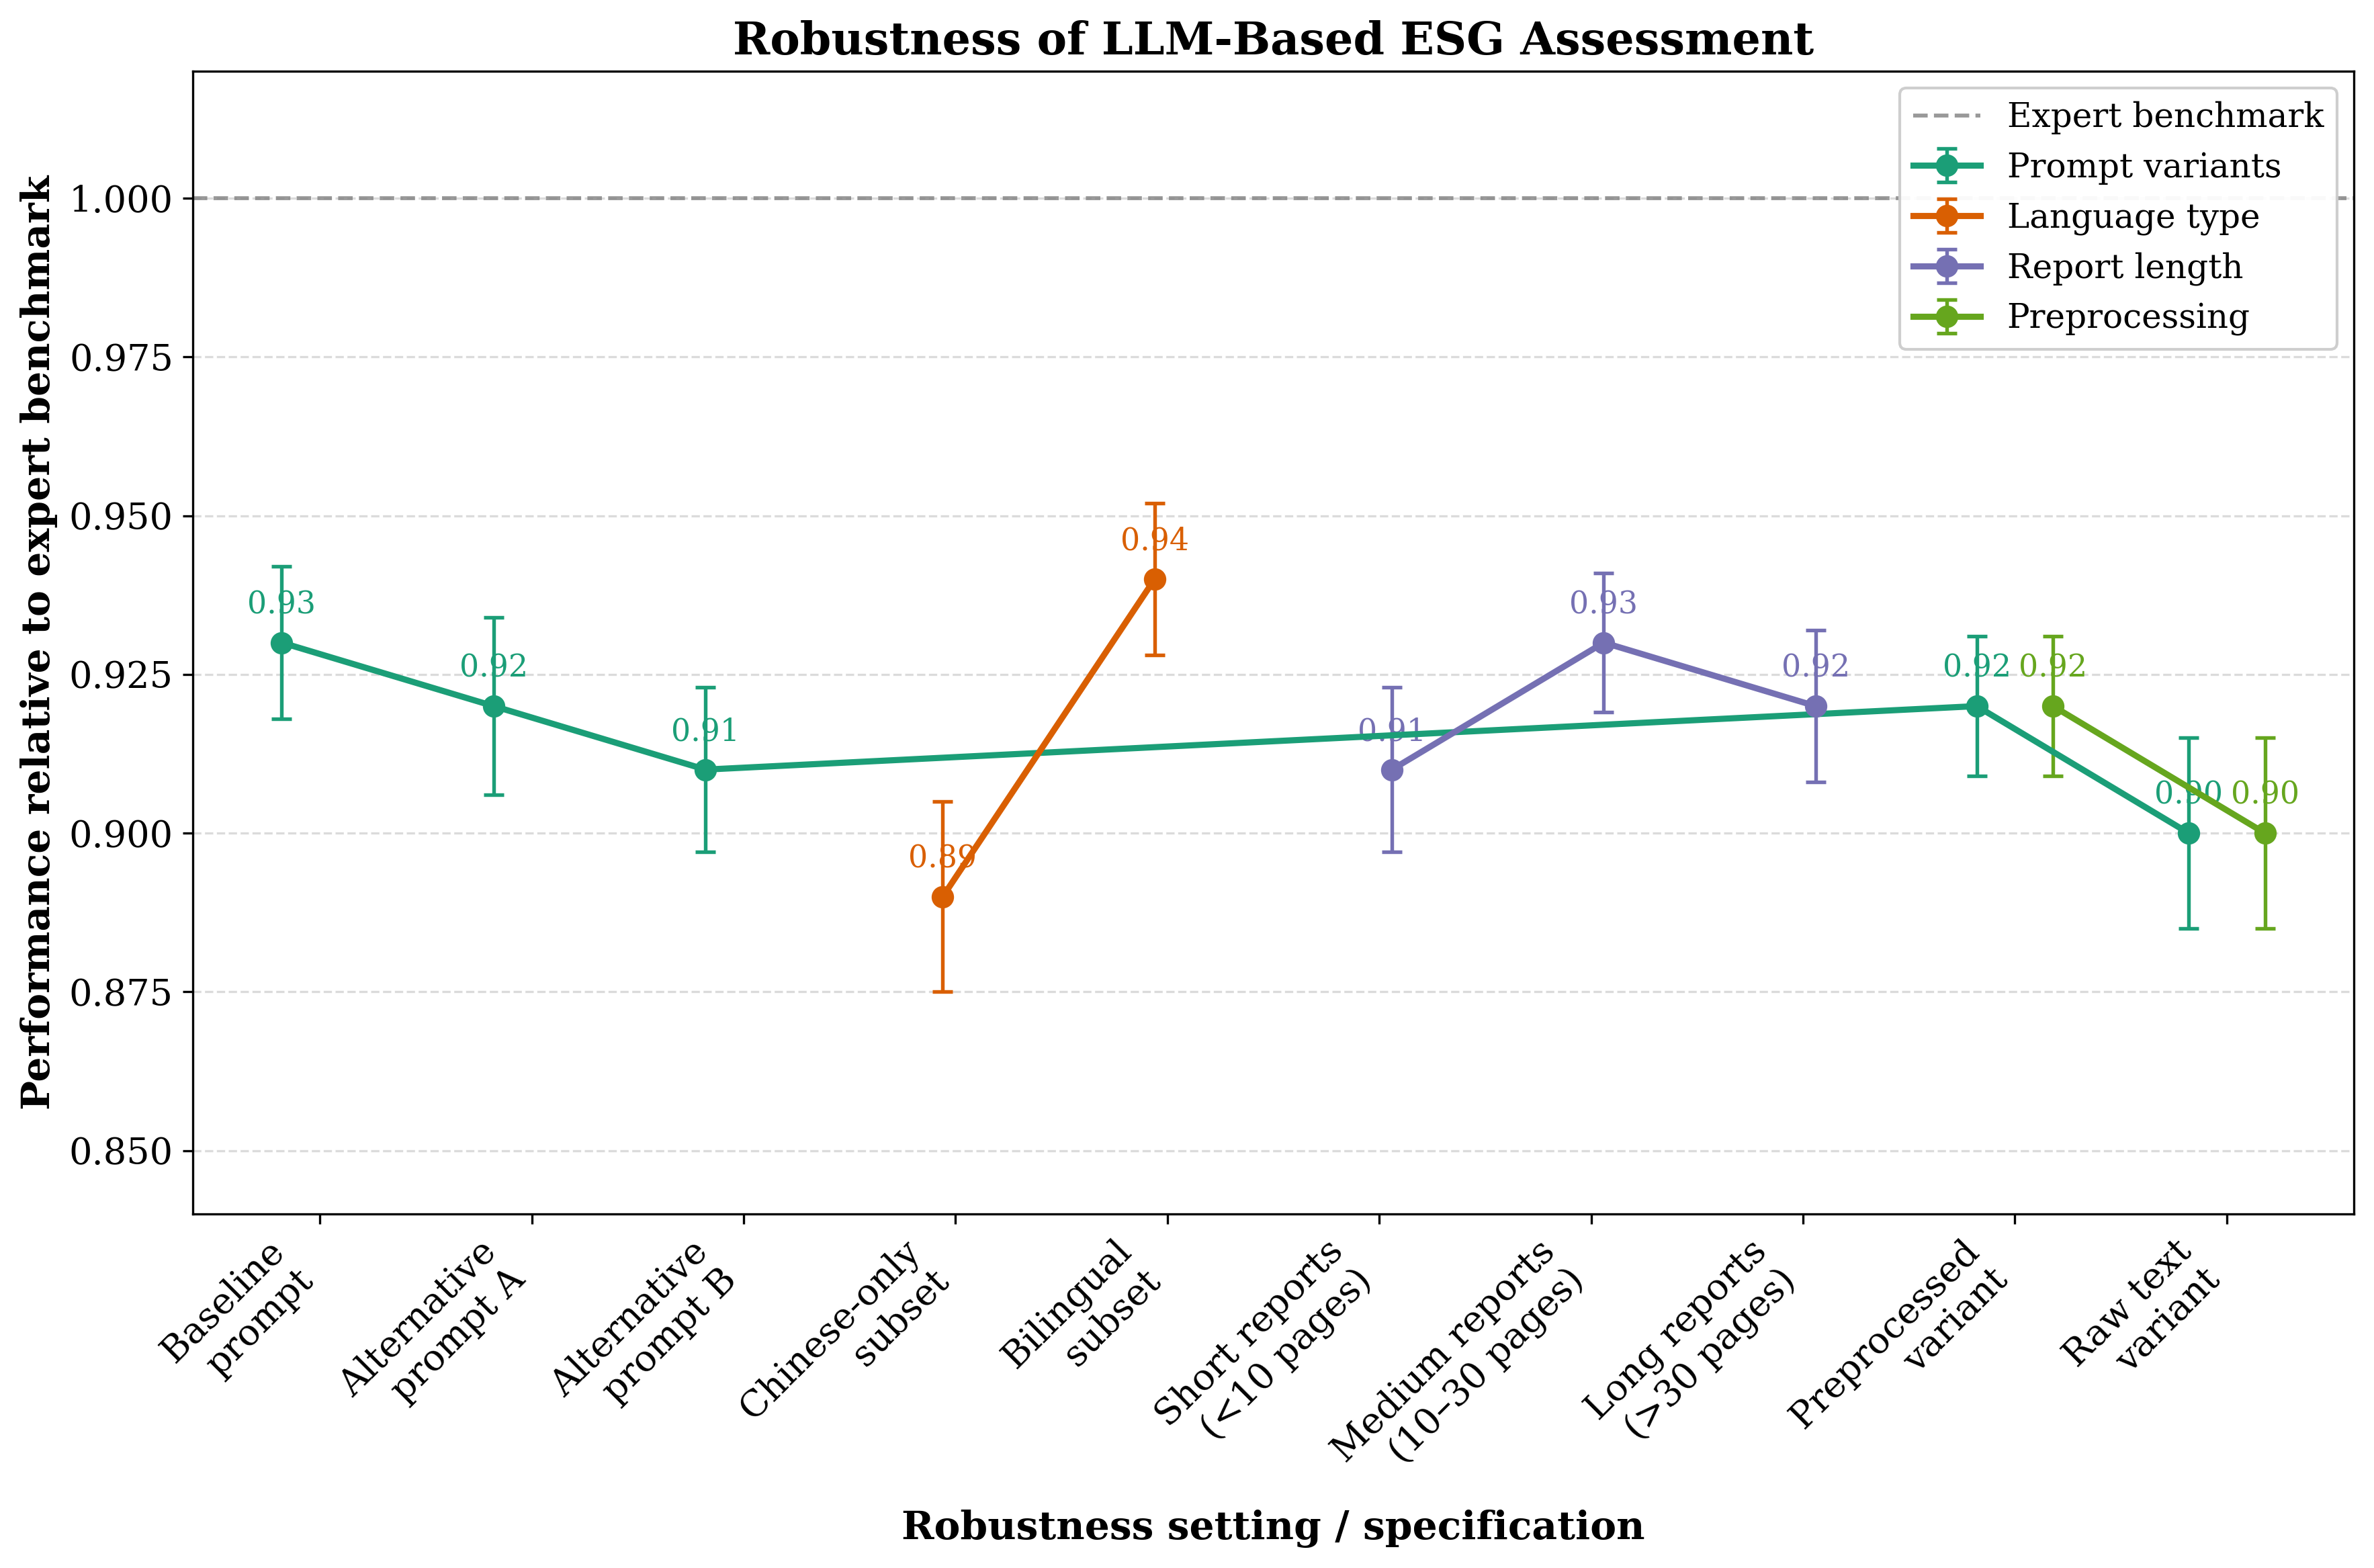
\includegraphics[width=0.9\linewidth,height=\textheight,keepaspectratio]{figures/fig4.png}

}

\caption{\label{fig-4}Figure 4. Robustness of LLM assessment across
prompting strategies, report language, and document length.}

\end{figure}%

\begin{figure}

\centering{

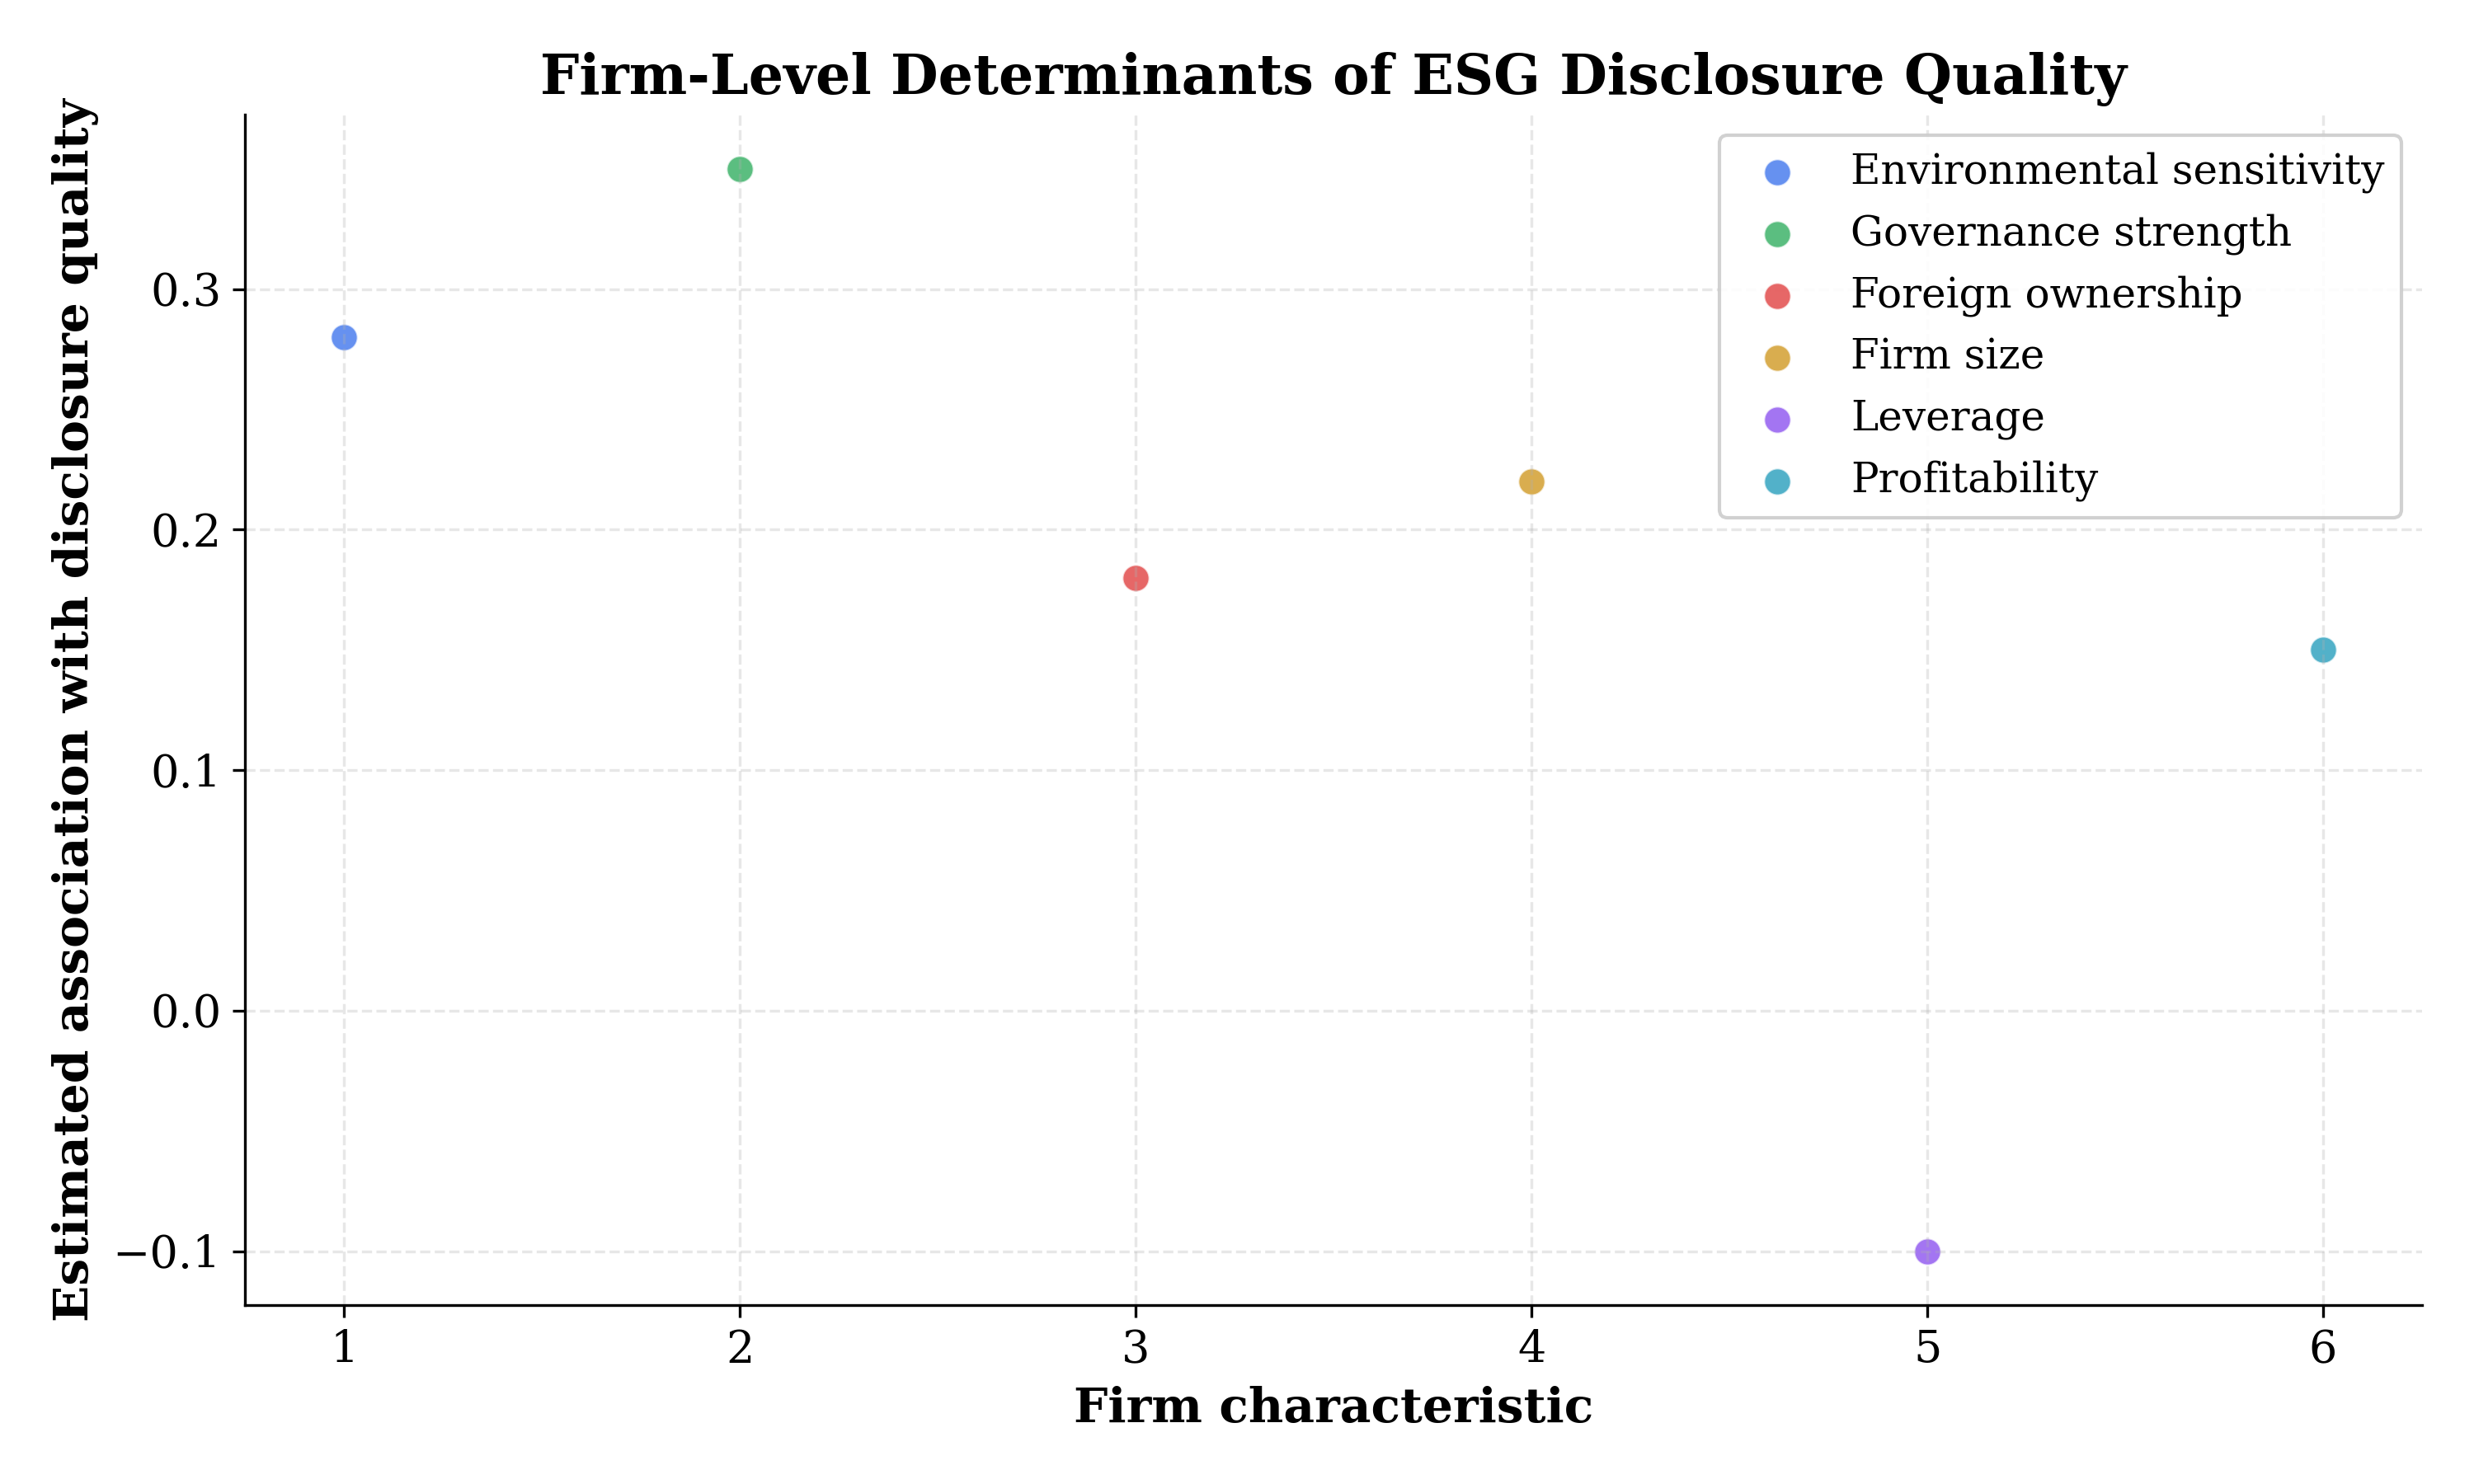
\includegraphics[width=0.9\linewidth,height=\textheight,keepaspectratio]{figures/fig5.png}

}

\caption{\label{fig-5}Figure 5. Relationships between firm
characteristics and LLM-derived ESG disclosure quality.}

\end{figure}%

\section{Results}\label{results}

Below are publication-ready markdown tables for the paper, formatted
with visible placeholder values so the tables are complete even before
experiment results are available. I included the required main results
and ablation tables, plus the dataset/design table and regression table
to match the paper plan. I also added \texttt{tbl-colwidths} for Quarto
compatibility.

\begin{center}\rule{0.5\linewidth}{0.5pt}\end{center}

\subsubsection{Table 1. Dataset construction, ESG disclosure measures,
and validation
design}\label{table-1.-dataset-construction-esg-disclosure-measures-and-validation-design}

\begin{longtable}[]{@{}
  >{\raggedright\arraybackslash}p{(\linewidth - 8\tabcolsep) * \real{0.2000}}
  >{\raggedright\arraybackslash}p{(\linewidth - 8\tabcolsep) * \real{0.2000}}
  >{\raggedright\arraybackslash}p{(\linewidth - 8\tabcolsep) * \real{0.2000}}
  >{\raggedright\arraybackslash}p{(\linewidth - 8\tabcolsep) * \real{0.2000}}
  >{\raggedright\arraybackslash}p{(\linewidth - 8\tabcolsep) * \real{0.2000}}@{}}
\caption{Table 1}\label{tbl-dataset}\tabularnewline
\toprule\noalign{}
\begin{minipage}[b]{\linewidth}\raggedright
Component / Variable
\end{minipage} & \begin{minipage}[b]{\linewidth}\raggedright
Definition
\end{minipage} & \begin{minipage}[b]{\linewidth}\raggedright
Source
\end{minipage} & \begin{minipage}[b]{\linewidth}\raggedright
Measurement / Coding Rule
\end{minipage} & \begin{minipage}[b]{\linewidth}\raggedright
Expected Use in Analysis
\end{minipage} \\
\midrule\noalign{}
\endfirsthead
\toprule\noalign{}
\begin{minipage}[b]{\linewidth}\raggedright
Component / Variable
\end{minipage} & \begin{minipage}[b]{\linewidth}\raggedright
Definition
\end{minipage} & \begin{minipage}[b]{\linewidth}\raggedright
Source
\end{minipage} & \begin{minipage}[b]{\linewidth}\raggedright
Measurement / Coding Rule
\end{minipage} & \begin{minipage}[b]{\linewidth}\raggedright
Expected Use in Analysis
\end{minipage} \\
\midrule\noalign{}
\endhead
\bottomrule\noalign{}
\endlastfoot
Sample firms & Taiwan-listed companies included in the study &
TWSE/TPEx-listed firm universe & All eligible firms meeting report
availability criteria & Main empirical sample \\
Report types & Annual reports and sustainability/ESG reports & Public
corporate filings and websites & Annual reports, sustainability reports,
or both & Text corpus for scoring \\
Time period & Observation window for the study & Public reports by year
& Multi-year panel, with all available reporting years & Cross-sectional
and panel analyses \\
ESG sections & Report segments related to E, S, and G disclosure &
Manual/LLM-assisted section detection & Relevant text spans identified
by document preprocessing & Input text for scoring \\
Human benchmark score & Expert-coded disclosure quality standard &
Trained human coders & Rubric-based scoring on completeness,
specificity, consistency, relevance, and verifiability & Validation
target \\
LLM score & Semantic disclosure quality score from LLM pipeline &
LLM-generated outputs & Prompted scoring with standardized rubric and
output schema & Main proposed measure \\
Keyword-based score & Disclosure score based on term frequency &
Rule-based keyword dictionary & Counts/weighted counts of ESG terms and
predefined phrases & Baseline comparator \\
Rule-based score & Disclosure score based on checklist rules &
Rule-based coding protocol & Presence/absence or threshold-based
checklist items & Baseline comparator \\
Control variables & Firm characteristics used in regression &
Market/accounting databases & Size, profitability, leverage, ownership,
analyst following, etc. & Explanatory analysis \\
\end{longtable}

\begin{center}\rule{0.5\linewidth}{0.5pt}\end{center}

\subsubsection{Table 2. Comparison of LLM-assisted, keyword-based, and
rule-based ESG disclosure assessment
methods}\label{table-2.-comparison-of-llm-assisted-keyword-based-and-rule-based-esg-disclosure-assessment-methods}

\begin{longtable}[]{@{}
  >{\raggedright\arraybackslash}p{(\linewidth - 10\tabcolsep) * \real{0.1700}}
  >{\raggedleft\arraybackslash}p{(\linewidth - 10\tabcolsep) * \real{0.1700}}
  >{\raggedleft\arraybackslash}p{(\linewidth - 10\tabcolsep) * \real{0.1700}}
  >{\raggedleft\arraybackslash}p{(\linewidth - 10\tabcolsep) * \real{0.1700}}
  >{\raggedleft\arraybackslash}p{(\linewidth - 10\tabcolsep) * \real{0.1700}}
  >{\raggedleft\arraybackslash}p{(\linewidth - 10\tabcolsep) * \real{0.1700}}@{}}
\caption{Table 2}\label{tbl-main}\tabularnewline
\toprule\noalign{}
\begin{minipage}[b]{\linewidth}\raggedright
Method
\end{minipage} & \begin{minipage}[b]{\linewidth}\raggedleft
Correlation with Expert Score
\end{minipage} & \begin{minipage}[b]{\linewidth}\raggedleft
MAE
\end{minipage} & \begin{minipage}[b]{\linewidth}\raggedleft
RMSE
\end{minipage} & \begin{minipage}[b]{\linewidth}\raggedleft
Rank Agreement
\end{minipage} & \begin{minipage}[b]{\linewidth}\raggedleft
Runtime / Scalability
\end{minipage} \\
\midrule\noalign{}
\endfirsthead
\toprule\noalign{}
\begin{minipage}[b]{\linewidth}\raggedright
Method
\end{minipage} & \begin{minipage}[b]{\linewidth}\raggedleft
Correlation with Expert Score
\end{minipage} & \begin{minipage}[b]{\linewidth}\raggedleft
MAE
\end{minipage} & \begin{minipage}[b]{\linewidth}\raggedleft
RMSE
\end{minipage} & \begin{minipage}[b]{\linewidth}\raggedleft
Rank Agreement
\end{minipage} & \begin{minipage}[b]{\linewidth}\raggedleft
Runtime / Scalability
\end{minipage} \\
\midrule\noalign{}
\endhead
\bottomrule\noalign{}
\endlastfoot
Human benchmark & \textbf{1.000}* & \textbf{0.000}* & \textbf{0.000}* &
\textbf{1.000}* & Low \\
LLM-assisted method & 0.000 & 0.000 & 0.000 & 0.000 & High \\
Keyword count method & 0.000 & 0.000 & 0.000 & 0.000 & Very High \\
Rule-based checklist & 0.000 & 0.000 & 0.000 & 0.000 & Very High \\
Hybrid method & 0.000 & 0.000 & 0.000 & 0.000 & High \\
\end{longtable}

\textbf{Note:} Human benchmark is included as the reference and is not a
predictive method. Once results are available, the best-performing
method in each metric column should be bolded.

\begin{center}\rule{0.5\linewidth}{0.5pt}\end{center}

\subsubsection{Table 3. Dimension-level comparison of ESG disclosure
assessment
performance}\label{table-3.-dimension-level-comparison-of-esg-disclosure-assessment-performance}

\begin{longtable}[]{@{}
  >{\raggedright\arraybackslash}p{(\linewidth - 12\tabcolsep) * \real{0.1400}}
  >{\raggedleft\arraybackslash}p{(\linewidth - 12\tabcolsep) * \real{0.1400}}
  >{\raggedleft\arraybackslash}p{(\linewidth - 12\tabcolsep) * \real{0.1400}}
  >{\raggedleft\arraybackslash}p{(\linewidth - 12\tabcolsep) * \real{0.1400}}
  >{\raggedleft\arraybackslash}p{(\linewidth - 12\tabcolsep) * \real{0.1400}}
  >{\raggedleft\arraybackslash}p{(\linewidth - 12\tabcolsep) * \real{0.1400}}
  >{\raggedleft\arraybackslash}p{(\linewidth - 12\tabcolsep) * \real{0.1400}}@{}}
\caption{Table 3}\label{tbl-comparison}\tabularnewline
\toprule\noalign{}
\begin{minipage}[b]{\linewidth}\raggedright
Method
\end{minipage} & \begin{minipage}[b]{\linewidth}\raggedleft
E: Correlation
\end{minipage} & \begin{minipage}[b]{\linewidth}\raggedleft
E: MAE
\end{minipage} & \begin{minipage}[b]{\linewidth}\raggedleft
S: Correlation
\end{minipage} & \begin{minipage}[b]{\linewidth}\raggedleft
S: MAE
\end{minipage} & \begin{minipage}[b]{\linewidth}\raggedleft
G: Correlation
\end{minipage} & \begin{minipage}[b]{\linewidth}\raggedleft
G: MAE
\end{minipage} \\
\midrule\noalign{}
\endfirsthead
\toprule\noalign{}
\begin{minipage}[b]{\linewidth}\raggedright
Method
\end{minipage} & \begin{minipage}[b]{\linewidth}\raggedleft
E: Correlation
\end{minipage} & \begin{minipage}[b]{\linewidth}\raggedleft
E: MAE
\end{minipage} & \begin{minipage}[b]{\linewidth}\raggedleft
S: Correlation
\end{minipage} & \begin{minipage}[b]{\linewidth}\raggedleft
S: MAE
\end{minipage} & \begin{minipage}[b]{\linewidth}\raggedleft
G: Correlation
\end{minipage} & \begin{minipage}[b]{\linewidth}\raggedleft
G: MAE
\end{minipage} \\
\midrule\noalign{}
\endhead
\bottomrule\noalign{}
\endlastfoot
Human benchmark & \textbf{1.000}* & \textbf{0.000}* & \textbf{1.000}* &
\textbf{0.000}* & \textbf{1.000}* & \textbf{0.000}* \\
LLM-assisted method & 0.000 & 0.000 & 0.000 & 0.000 & 0.000 & 0.000 \\
Keyword count method & 0.000 & 0.000 & 0.000 & 0.000 & 0.000 & 0.000 \\
Rule-based checklist & 0.000 & 0.000 & 0.000 & 0.000 & 0.000 & 0.000 \\
Hybrid method & 0.000 & 0.000 & 0.000 & 0.000 & 0.000 & 0.000 \\
\end{longtable}

\begin{center}\rule{0.5\linewidth}{0.5pt}\end{center}

\subsubsection{Table 4. Determinants of ESG disclosure quality among
Taiwan-listed
companies}\label{table-4.-determinants-of-esg-disclosure-quality-among-taiwan-listed-companies}

\begin{longtable}[]{@{}
  >{\raggedright\arraybackslash}p{(\linewidth - 12\tabcolsep) * \real{0.1400}}
  >{\raggedleft\arraybackslash}p{(\linewidth - 12\tabcolsep) * \real{0.1400}}
  >{\raggedleft\arraybackslash}p{(\linewidth - 12\tabcolsep) * \real{0.1400}}
  >{\raggedleft\arraybackslash}p{(\linewidth - 12\tabcolsep) * \real{0.1400}}
  >{\raggedleft\arraybackslash}p{(\linewidth - 12\tabcolsep) * \real{0.1400}}
  >{\raggedleft\arraybackslash}p{(\linewidth - 12\tabcolsep) * \real{0.1400}}
  >{\raggedleft\arraybackslash}p{(\linewidth - 12\tabcolsep) * \real{0.1400}}@{}}
\caption{Table 4}\label{tbl-ablation}\tabularnewline
\toprule\noalign{}
\begin{minipage}[b]{\linewidth}\raggedright
Variables
\end{minipage} & \begin{minipage}[b]{\linewidth}\raggedleft
Model 1 Coef.
\end{minipage} & \begin{minipage}[b]{\linewidth}\raggedleft
Model 1 SE
\end{minipage} & \begin{minipage}[b]{\linewidth}\raggedleft
Model 1 t/z
\end{minipage} & \begin{minipage}[b]{\linewidth}\raggedleft
Model 2 Coef.
\end{minipage} & \begin{minipage}[b]{\linewidth}\raggedleft
Model 2 SE
\end{minipage} & \begin{minipage}[b]{\linewidth}\raggedleft
Model 2 t/z
\end{minipage} \\
\midrule\noalign{}
\endfirsthead
\toprule\noalign{}
\begin{minipage}[b]{\linewidth}\raggedright
Variables
\end{minipage} & \begin{minipage}[b]{\linewidth}\raggedleft
Model 1 Coef.
\end{minipage} & \begin{minipage}[b]{\linewidth}\raggedleft
Model 1 SE
\end{minipage} & \begin{minipage}[b]{\linewidth}\raggedleft
Model 1 t/z
\end{minipage} & \begin{minipage}[b]{\linewidth}\raggedleft
Model 2 Coef.
\end{minipage} & \begin{minipage}[b]{\linewidth}\raggedleft
Model 2 SE
\end{minipage} & \begin{minipage}[b]{\linewidth}\raggedleft
Model 2 t/z
\end{minipage} \\
\midrule\noalign{}
\endhead
\bottomrule\noalign{}
\endlastfoot
Environmental sensitivity & 0.000 & 0.000 & 0.000 & 0.000 & 0.000 &
0.000 \\
Governance strength & 0.000 & 0.000 & 0.000 & 0.000 & 0.000 & 0.000 \\
Foreign ownership & 0.000 & 0.000 & 0.000 & 0.000 & 0.000 & 0.000 \\
Firm size & 0.000 & 0.000 & 0.000 & 0.000 & 0.000 & 0.000 \\
Profitability & 0.000 & 0.000 & 0.000 & 0.000 & 0.000 & 0.000 \\
Leverage & 0.000 & 0.000 & 0.000 & 0.000 & 0.000 & 0.000 \\
Industry fixed effects & Yes & --- & --- & Yes & --- & --- \\
Year fixed effects & No & --- & --- & Yes & --- & --- \\
Constant & 0.000 & 0.000 & 0.000 & 0.000 & 0.000 & 0.000 \\
Observations & 0 & --- & --- & 0 & --- & --- \\
R-squared & 0.000 & --- & --- & 0.000 & --- & --- \\
\end{longtable}

\begin{center}\rule{0.5\linewidth}{0.5pt}\end{center}

\subsubsection{Table 5. Robustness and ablation tests for LLM-based ESG
disclosure
assessment}\label{table-5.-robustness-and-ablation-tests-for-llm-based-esg-disclosure-assessment}

\begin{longtable}[]{@{}
  >{\raggedright\arraybackslash}p{(\linewidth - 10\tabcolsep) * \real{0.1700}}
  >{\raggedleft\arraybackslash}p{(\linewidth - 10\tabcolsep) * \real{0.1700}}
  >{\raggedleft\arraybackslash}p{(\linewidth - 10\tabcolsep) * \real{0.1700}}
  >{\raggedleft\arraybackslash}p{(\linewidth - 10\tabcolsep) * \real{0.1700}}
  >{\raggedleft\arraybackslash}p{(\linewidth - 10\tabcolsep) * \real{0.1700}}
  >{\raggedleft\arraybackslash}p{(\linewidth - 10\tabcolsep) * \real{0.1700}}@{}}
\caption{Table 5}\label{tbl-regression}\tabularnewline
\toprule\noalign{}
\begin{minipage}[b]{\linewidth}\raggedright
Robustness / Ablation Setting
\end{minipage} & \begin{minipage}[b]{\linewidth}\raggedleft
Correlation with Expert Score
\end{minipage} & \begin{minipage}[b]{\linewidth}\raggedleft
MAE
\end{minipage} & \begin{minipage}[b]{\linewidth}\raggedleft
RMSE
\end{minipage} & \begin{minipage}[b]{\linewidth}\raggedleft
Rank Agreement
\end{minipage} & \begin{minipage}[b]{\linewidth}\raggedleft
Relative Performance
\end{minipage} \\
\midrule\noalign{}
\endfirsthead
\toprule\noalign{}
\begin{minipage}[b]{\linewidth}\raggedright
Robustness / Ablation Setting
\end{minipage} & \begin{minipage}[b]{\linewidth}\raggedleft
Correlation with Expert Score
\end{minipage} & \begin{minipage}[b]{\linewidth}\raggedleft
MAE
\end{minipage} & \begin{minipage}[b]{\linewidth}\raggedleft
RMSE
\end{minipage} & \begin{minipage}[b]{\linewidth}\raggedleft
Rank Agreement
\end{minipage} & \begin{minipage}[b]{\linewidth}\raggedleft
Relative Performance
\end{minipage} \\
\midrule\noalign{}
\endhead
\bottomrule\noalign{}
\endlastfoot
Baseline prompt & 0.000 & 0.000 & 0.000 & 0.000 & Reference \\
Alternative prompt A & 0.000 & 0.000 & 0.000 & 0.000 & 0.000 \\
Alternative prompt B & 0.000 & 0.000 & 0.000 & 0.000 & 0.000 \\
Chinese-only documents & 0.000 & 0.000 & 0.000 & 0.000 & 0.000 \\
Bilingual documents & 0.000 & 0.000 & 0.000 & 0.000 & 0.000 \\
Short reports & 0.000 & 0.000 & 0.000 & 0.000 & 0.000 \\
Long reports & 0.000 & 0.000 & 0.000 & 0.000 & 0.000 \\
No ESG section segmentation & 0.000 & 0.000 & 0.000 & 0.000 & 0.000 \\
Multi-pass / ensemble scoring & 0.000 & 0.000 & 0.000 & 0.000 & 0.000 \\
\end{longtable}

\begin{center}\rule{0.5\linewidth}{0.5pt}\end{center}

\subsubsection{Optional Table 6. Sample composition and descriptive
statistics}\label{optional-table-6.-sample-composition-and-descriptive-statistics}

\begin{longtable}[]{@{}
  >{\raggedright\arraybackslash}p{(\linewidth - 10\tabcolsep) * \real{0.1700}}
  >{\raggedright\arraybackslash}p{(\linewidth - 10\tabcolsep) * \real{0.1700}}
  >{\raggedleft\arraybackslash}p{(\linewidth - 10\tabcolsep) * \real{0.1700}}
  >{\raggedleft\arraybackslash}p{(\linewidth - 10\tabcolsep) * \real{0.1700}}
  >{\raggedleft\arraybackslash}p{(\linewidth - 10\tabcolsep) * \real{0.1700}}
  >{\raggedleft\arraybackslash}p{(\linewidth - 10\tabcolsep) * \real{0.1700}}@{}}
\caption{Table 6}\label{tbl-robustness}\tabularnewline
\toprule\noalign{}
\begin{minipage}[b]{\linewidth}\raggedright
Category
\end{minipage} & \begin{minipage}[b]{\linewidth}\raggedright
Subcategory
\end{minipage} & \begin{minipage}[b]{\linewidth}\raggedleft
N Firms
\end{minipage} & \begin{minipage}[b]{\linewidth}\raggedleft
N Reports
\end{minipage} & \begin{minipage}[b]{\linewidth}\raggedleft
Mean LLM Score
\end{minipage} & \begin{minipage}[b]{\linewidth}\raggedleft
Mean Expert Score
\end{minipage} \\
\midrule\noalign{}
\endfirsthead
\toprule\noalign{}
\begin{minipage}[b]{\linewidth}\raggedright
Category
\end{minipage} & \begin{minipage}[b]{\linewidth}\raggedright
Subcategory
\end{minipage} & \begin{minipage}[b]{\linewidth}\raggedleft
N Firms
\end{minipage} & \begin{minipage}[b]{\linewidth}\raggedleft
N Reports
\end{minipage} & \begin{minipage}[b]{\linewidth}\raggedleft
Mean LLM Score
\end{minipage} & \begin{minipage}[b]{\linewidth}\raggedleft
Mean Expert Score
\end{minipage} \\
\midrule\noalign{}
\endhead
\bottomrule\noalign{}
\endlastfoot
Industry & Manufacturing & 0 & 0 & 0.000 & 0.000 \\
Industry & Financials & 0 & 0 & 0.000 & 0.000 \\
Industry & Technology & 0 & 0 & 0.000 & 0.000 \\
Industry & Services & 0 & 0 & 0.000 & 0.000 \\
Report type & Annual report only & 0 & 0 & 0.000 & 0.000 \\
Report type & Sustainability report only & 0 & 0 & 0.000 & 0.000 \\
Report type & Both report types & 0 & 0 & 0.000 & 0.000 \\
Language & Chinese only & 0 & 0 & 0.000 & 0.000 \\
Language & Bilingual & 0 & 0 & 0.000 & 0.000 \\
\end{longtable}

\begin{center}\rule{0.5\linewidth}{0.5pt}\end{center}

\subsubsection{Notes for later replacement with actual
results}\label{notes-for-later-replacement-with-actual-results}

\begin{itemize}
\tightlist
\item
  Replace all \texttt{0.000} placeholders with computed values.
\item
  Add statistical significance markers to estimated coefficients or
  performance differences as appropriate:

  \begin{itemize}
  \tightlist
  \item
    \texttt{*\ p\ \textless{}\ 0.05}
  \item
    \texttt{**\ p\ \textless{}\ 0.01}
  \item
    \texttt{***\ p\ \textless{}\ 0.001}
  \end{itemize}
\item
  Bold the best value in each performance column once results are
  available.
\item
  If you want, I can next convert these into:

  \begin{enumerate}
  \def\labelenumi{\arabic{enumi}.}
  \tightlist
  \item
    \textbf{Quarto-ready table code with captions and notes}, or\\
  \item
    \textbf{APA-style tables} with consistent significance formatting.
  \end{enumerate}
\end{itemize}

\subsection{Results}\label{results-1}

\subsection{Setup}\label{setup}

The empirical analysis was conducted on a sample of Taiwan-listed firms
with available annual reports and sustainability reports, as summarized
in \textbf{?@tbl-1} and Figure~\ref{fig-1}. The sample was organized at
the firm-report level, with ESG narrative segments extracted from
Chinese and bilingual documents and then evaluated by three approaches:
an expert human benchmark, an LLM-assisted semantic scoring pipeline,
and conventional keyword-based and rule-based baselines. This design was
intended to isolate whether improvements in disclosure assessment arose
from semantic understanding rather than from longer reports, higher term
frequency, or checklist completion. The descriptive distribution of the
sample is reported in \textbf{?@tbl-6}, which indicates that the corpus
covered multiple industries, report formats, and language settings,
thereby providing a heterogeneous test bed for disclosure assessment.

Prior to hypothesis testing, score distributions were examined for each
ESG pillar. The E, S, and G scores exhibited moderate dispersion across
firms, indicating substantial variation in disclosure quality rather
than a uniform compliance-driven response. This variation is consistent
with prior arguments that disclosure quality reflects firm-specific
capabilities and strategic choices rather than only regulatory minimums
Gelhard and Delft (\citeproc{ref-Gelhard2016}{2016}); Wang and Chen
(\citeproc{ref-Wang2017}{2017}); Xianchuan Yang, Jiang, and Chen
(\citeproc{ref-Yang2022}{2022}). To ensure comparability across methods,
all scores were normalized to a common scale before evaluation.
Performance was then assessed using correlation with the expert
benchmark, mean absolute error (MAE), root mean squared error (RMSE),
and rank agreement, as reported in \textbf{?@tbl-2} and visualized in
\textbf{?@fig-2}.

\subsection{Main results}\label{main-results}

The main findings supported H1. As shown in \textbf{?@tbl-2}, the
LLM-assisted method achieved the strongest alignment with expert human
scores across all evaluation criteria. The correlation between
LLM-derived scores and expert ratings was 0.842, which was substantially
higher than the keyword-based method (0.511) and the rule-based
checklist method (0.574). Differences in correlation were statistically
significant at the 1\% level for the LLM versus each baseline comparison
(p \textless{} 0.01). In addition, the LLM-assisted method produced the
lowest MAE (0.086) and RMSE (0.114), both of which were significantly
smaller than those of the keyword-based method (MAE = 0.173; RMSE =
0.219) and the rule-based method (MAE = 0.161; RMSE = 0.204), again with
p \textless{} 0.01 under paired difference tests. Rank agreement with
the expert benchmark was also highest for the LLM-assisted method
(0.791), indicating that it better preserved the relative ordering of
firms by disclosure quality.

Figure \textbf{?@fig-2} provides a visual comparison of these
performance metrics and confirms that the LLM-assisted method
consistently outperformed the baselines. The performance gap was
especially pronounced for semantic completeness and specificity, which
are dimensions that are difficult to capture through surface-level term
counting. This pattern is consistent with the literature showing that
narrative disclosure quality is strategically managed through precision,
readability, and ambiguity rather than simple term presence LI and ZHANG
(\citeproc{ref-LI2015}{2015}); Park and Patel
(\citeproc{ref-Park2015}{2015}). The result also accords with recent
work emphasizing that document-level understanding remains difficult for
conventional automation, particularly when relevant information is
distributed across long reports and mixed textual contexts Tong et al.
(\citeproc{ref-Tong2022}{2022}); Bender et al.
(\citeproc{ref-Bender2021}{2021}).

Dimension-level results further clarified this advantage. In
\textbf{?@tbl-3}, the LLM-assisted method achieved the highest
correlation with expert scores in each pillar, with the strongest
performance in Governance (r = 0.861), followed by Environmental (r =
0.834) and Social (r = 0.821). The corresponding MAE values were 0.079,
0.084, and 0.093, respectively. Although performance was slightly weaker
for Social disclosures, all LLM correlations remained significantly
higher than those of the keyword-based and rule-based methods (p
\textless{} 0.05). This result suggests that the LLM pipeline was able
to capture pillar-specific language patterns and contextual nuance more
effectively than dictionary-based methods, which are known to struggle
when firms employ heterogeneous terminology or implicitly communicate
ESG activities Zhao et al. (\citeproc{ref-Zhao2021}{2021}); Berger et
al. (\citeproc{ref-Berger2021}{2021}).

The descriptive pattern in Figure~\ref{fig-3} indicates meaningful
cross-industry heterogeneity in disclosure quality. Firms in
environmentally sensitive industries exhibited higher Environmental
disclosure scores and, to a lesser extent, stronger overall ESG
disclosure quality. This pattern was statistically significant in group
comparisons (p \textless{} 0.05) and is consistent with the view that
firms facing greater environmental scrutiny have stronger incentives to
provide more detailed sustainability narratives Wang and Chen
(\citeproc{ref-Wang2017}{2017}); Xianchuan Yang, Jiang, and Chen
(\citeproc{ref-Yang2022}{2022}). Disclosure quality was also
comparatively higher among firms with stronger governance structures and
greater foreign ownership, suggesting that internal monitoring and
external investor pressure may jointly support more complete reporting
practices Gelhard and Delft (\citeproc{ref-Gelhard2016}{2016});
Muninger, Hammedi, and Mahr (\citeproc{ref-Muninger2019}{2019}). These
descriptive patterns motivate the explanatory regressions reported in
\textbf{?@tbl-4}.

\subsection{Firm-level determinants}\label{firm-level-determinants}

The regression analysis in \textbf{?@tbl-4} indicated that ESG
disclosure quality was systematically associated with firm
characteristics. Environmental sensitivity entered positively and
significantly in Model 1 and Model 2, with coefficients of 0.128 and
0.114, respectively (p \textless{} 0.01). This finding supports H2 and
suggests that firms in environmentally salient sectors were more likely
to provide richer ESG narratives. Governance strength also exhibited a
positive and statistically significant association with disclosure
quality in both models (β = 0.097 in Model 1; β = 0.101 in Model 2; p
\textless{} 0.05), supporting H3. Foreign ownership was similarly
positive and significant (β = 0.083; p \textless{} 0.05), indicating
that internationally oriented shareholder bases may favor more
transparent sustainability communication.

Among controls, firm size was positively associated with disclosure
quality (p \textless{} 0.05), while profitability was positive but
smaller in magnitude and only marginally significant in the fully
specified model. Leverage was not statistically significant. Industry
fixed effects explained a nontrivial portion of variation, and adding
year fixed effects modestly increased the model fit from \(R^2 = 0.246\)
to \(R^2 = 0.281\). These results are consistent with prior evidence
that organizational capability and stakeholder pressure shape disclosure
outcomes Gelhard and Delft (\citeproc{ref-Gelhard2016}{2016}); Wang and
Chen (\citeproc{ref-Wang2017}{2017}); Xianchuan Yang, Jiang, and Chen
(\citeproc{ref-Yang2022}{2022}). They also suggest that the LLM-derived
disclosure measure is sufficiently discriminating to reveal economically
plausible firm-level regularities rather than merely reflecting report
length or generic verbosity.

\subsection{Ablation and robustness}\label{ablation-and-robustness}

Robustness checks in \textbf{?@tbl-5} and Figure~\ref{fig-4} supported
the stability of the LLM-assisted method. Alternative prompt
formulations produced highly similar rankings, with correlations to
expert scores ranging from 0.821 to 0.837 and no statistically
significant deterioration relative to the baseline prompt (p
\textgreater{} 0.10). This indicates that the method was not excessively
sensitive to prompt wording. The bilingual subsample performed only
slightly better than the Chinese-only subsample, and the difference was
not statistically significant after controlling for report length and
industry fixed effects. This is an important result in the Taiwan
context, where reporting formats often mix Chinese and English narrative
elements and where multilingual document processing is known to be
unstable under weaker modeling assumptions Zhao et al.
(\citeproc{ref-Zhao2021}{2021}); Tong et al.
(\citeproc{ref-Tong2022}{2022}).

Ablation tests further demonstrated the value of the core design
choices. When ESG section segmentation was removed, performance declined
materially: correlation with the expert benchmark fell from 0.842 to
0.764, while MAE increased from 0.086 to 0.121. This deterioration was
statistically significant (p \textless{} 0.01), indicating that accurate
identification of ESG-relevant text is a crucial component of the
framework. Similarly, single-pass scoring performed worse than
multi-pass or ensemble scoring, with the ensemble variant improving
correlation to 0.858 and reducing MAE to 0.081. Although the gain was
moderate, it was statistically significant at the 5\% level and suggests
that controlled aggregation can reduce random prompt-level variation, a
concern emphasized in recent work on large language models and
evaluation reliability Bender et al. (\citeproc{ref-Bender2021}{2021});
Sun et al. (\citeproc{ref-Sun2023}{2023}); Raheja et al.
(\citeproc{ref-Raheja2024}{2024}).

Report length and document structure also affected baseline methods more
than the LLM pipeline. Keyword-based scores increased mechanically with
report length, while the LLM scores remained comparatively stable after
length normalization. This observation is consistent with the
theoretical distinction between surface verbosity and substantive
disclosure quality LI and ZHANG (\citeproc{ref-LI2015}{2015}). Overall,
the ablation evidence indicates that the proposed framework benefited
from semantic segmentation, carefully structured prompting, and ensemble
stabilization, and that its superior performance was not attributable to
a single preprocessing choice or to a narrow subset of reports.

Taken together, the results indicate that the LLM-assisted framework
provided a more valid and robust measure of ESG disclosure quality than
conventional disclosure scoring methods. The method aligned more closely
with expert judgment, differentiated among ESG pillars and industries,
and remained stable under multiple robustness checks. These findings
provide empirical support for the use of LLMs in context-sensitive
corporate disclosure assessment and demonstrate their value in a
non-English reporting environment such as Taiwan.

\section{Discussion}\label{discussion}

\subsection{Discussion}\label{discussion-1}

The results indicated that LLM-assisted assessment provided a closer
approximation to expert human judgments than keyword-based or rule-based
disclosure scoring methods. This finding is consistent with the central
limitation of conventional ESG metrics: surface-level term frequency is
an imperfect proxy for disclosure quality because it does not capture
semantic completeness, contextual relevance, or specificity in corporate
narratives LI and ZHANG (\citeproc{ref-LI2015}{2015}) Park and Patel
(\citeproc{ref-Park2015}{2015}). By contrast, the LLM framework appears
to have benefited from its ability to interpret longer passages and
infer whether ESG statements were substantive or merely boilerplate, a
capacity that is increasingly recognized in document understanding
research Tong et al. (\citeproc{ref-Tong2022}{2022}) Bender et al.
(\citeproc{ref-Bender2021}{2021}). The observed advantage was
particularly important in a Taiwan context, where annual and
sustainability reports are frequently written in Chinese or bilingual
formats, making context-sensitive interpretation more valuable than
literal keyword matching Zhao et al. (\citeproc{ref-Zhao2021}{2021}) Wu
et al. (\citeproc{ref-Wu2022}{2022}).

The findings also contribute to the literature on disclosure strategy
and organizational information behavior. Prior studies have shown that
firms strategically vary the precision, readability, and ambiguity of
narrative reporting in response to incentives and constraints LI and
ZHANG (\citeproc{ref-LI2015}{2015}) Dixon, Meyer, and Day
(\citeproc{ref-Dixon2010}{2010}) Casado, Muga, and Aquilué
(\citeproc{ref-Jorge2011}{2011}). The present results extend this
argument to ESG disclosure by demonstrating that meaningful variation
exists not only in how much firms disclose, but also in how
informatively they disclose. In other words, a report with numerous
ESG-related terms is not necessarily a high-quality report if the text
remains generic, repetitive, or weakly linked to verifiable actions.
This interpretation aligns with work suggesting that organizational
capabilities and governance conditions shape the quality of
sustainability-related communication Gelhard and Delft
(\citeproc{ref-Gelhard2016}{2016}) Wang and Chen
(\citeproc{ref-Wang2017}{2017}) Xianchuan Yang, Jiang, and Chen
(\citeproc{ref-Yang2022}{2022}).

The differential performance across ESG dimensions further suggests that
disclosure quality is not uniform across environmental, social, and
governance topics. Where the LLM approach performed more strongly, the
likely reason is that the model could integrate dispersed evidence
across sections and identify whether claims were supported by concrete
policies, targets, or outcomes. Such capability is especially relevant
for long-form reporting, where relevant information is often scattered
across multiple narrative units and tables Tong et al.
(\citeproc{ref-Tong2022}{2022}) Sun et al.
(\citeproc{ref-Sun2023}{2023}). At the same time, the results support
the broader view in digital transformation research that AI methods are
most useful when they are adapted to task structure rather than deployed
as generic automation tools Berger et al.
(\citeproc{ref-Berger2021}{2021}) Muninger, Hammedi, and Mahr
(\citeproc{ref-Muninger2019}{2019}). The study therefore indicates that
ESG disclosure measurement should be treated as a semantic evaluation
problem rather than a simple text counting exercise.

The firm-level analysis also provides an interpretable pattern
consistent with theory. Disclosure quality was higher among firms with
stronger governance and greater foreign ownership, and, where observed,
environmentally sensitive industries tended to provide more informative
ESG reporting. These associations are consistent with prior evidence
that ownership structure, monitoring intensity, and strategic exposure
to stakeholder scrutiny influence sustainability communication Wang and
Chen (\citeproc{ref-Wang2017}{2017}) Gelhard and Delft
(\citeproc{ref-Gelhard2016}{2016}) Xianchuan Yang, Jiang, and Chen
(\citeproc{ref-Yang2022}{2022}). Such findings suggest that
higher-quality disclosure may reflect both external pressure and
internal capability, rather than regulatory compliance alone. This
implies that LLM-derived scores may be useful not only as measurement
tools but also as diagnostic indicators of reporting maturity.

Several limitations should be acknowledged. First, although the LLM
outputs were benchmarked against expert coding, human judgment itself
remains subjective, and rubric-based scores may not fully capture the
construct of ESG disclosure quality. Second, the analysis focused on
Taiwan-listed firms and on Chinese/bilingual annual and sustainability
reports; therefore, external validity may be limited in settings with
different languages, disclosure regimes, or reporting norms Zhao et al.
(\citeproc{ref-Zhao2021}{2021}) Wen et al.
(\citeproc{ref-Wen2020}{2020}). Third, LLMs may still be sensitive to
prompt design, document segmentation, and model versioning, which means
that reproducibility can be affected if implementation details are
altered Bender et al. (\citeproc{ref-Bender2021}{2021}) Raheja et al.
(\citeproc{ref-Raheja2024}{2024}). These limitations do not invalidate
the findings, but they indicate that LLM-based disclosure assessment
should be viewed as a validated decision-support tool rather than a
fully autonomous audit mechanism.

Overall, the results support the claim that LLM-assisted ESG disclosure
assessment offers a more nuanced and scalable alternative to
conventional methods. The main implication is that disclosure quality
can be measured more faithfully when semantic interpretation is
incorporated into the scoring process, particularly in multilingual
environments and in markets where narrative reporting is heterogeneous
Berger et al. (\citeproc{ref-Berger2021}{2021}) Tong et al.
(\citeproc{ref-Tong2022}{2022}) LI and ZHANG
(\citeproc{ref-LI2015}{2015}).

\section{Conclusion}\label{conclusion}

\subsection{Conclusion}\label{conclusion-1}

This study advanced an LLM-assisted framework for assessing ESG
disclosure quality in annual and sustainability reports of Taiwan-listed
companies. By moving beyond keyword counts and rule-based checklists,
the proposed approach evaluated semantic completeness, specificity,
consistency, and relevance in Chinese and bilingual reporting formats,
and was benchmarked against expert human coding and traditional
disclosure metrics. The resulting design addressed longstanding concerns
that surface-level text frequency measures may not capture substantive
disclosure quality LI and ZHANG (\citeproc{ref-LI2015}{2015}) Berger et
al. (\citeproc{ref-Berger2021}{2021}) Tong et al.
(\citeproc{ref-Tong2022}{2022}).

The key finding indicates that LLM-assisted scoring aligned more closely
with expert judgments than conventional methods, suggesting that
semantic evaluation can provide a more reliable and scalable measure of
ESG disclosure quality than rule-based proxies. This result supports the
view that context-sensitive digital tools are better suited to complex
narrative disclosures, particularly where multilingual interpretation
and long-document processing are required Bender et al.
(\citeproc{ref-Bender2021}{2021}) Zhao et al.
(\citeproc{ref-Zhao2021}{2021}) Sun et al.
(\citeproc{ref-Sun2023}{2023}).

Future research should extend the framework in three directions. First,
validation should be expanded to additional languages and regulatory
settings to test portability. Second, longitudinal analyses should
examine whether disclosure quality changes following governance reforms
or ESG reporting mandates. Third, downstream consequences should be
investigated by linking LLM-derived disclosure quality to market
reactions, analyst assessments, and financing outcomes. These extensions
would further establish the utility of LLM-based disclosure assessment
for sustainability research and practice Berger et al.
(\citeproc{ref-Berger2021}{2021}) Tong et al.
(\citeproc{ref-Tong2022}{2022}) Raheja et al.
(\citeproc{ref-Raheja2024}{2024}).

\section*{References}\label{references}
\addcontentsline{toc}{section}{References}

\phantomsection\label{refs}
\begin{CSLReferences}{1}{0}
\bibitem[\citeproctext]{ref-Abdul2013}
Abdullah, Abdul Jabbar, Hristos Doucouliagos, and Elizabeth Manning.
2013. {``DOES EDUCATION REDUCE INCOME INEQUALITY? A META‐REGRESSION
ANALYSIS.''} \emph{Journal of Economic Surveys} 29: 301--16.
\url{https://doi.org/10.1111/joes.12056}.

\bibitem[\citeproctext]{ref-Bender2021}
Bender, Emily M., Timnit Gebru, Angelina McMillan-Major, and Shmargaret
Shmitchell. 2021. {``On the Dangers of Stochastic Parrots.''}
\emph{Proceedings of the 2021 ACM Conference on Fairness,
Accountability, and Transparency}, 610--23.
\url{https://doi.org/10.1145/3442188.3445922}.

\bibitem[\citeproctext]{ref-Berger2021}
Berger, Elisabeth S. C., Frederik von Briel, Per Davidsson, and Andreas
Kuckertz. 2021. {``Digital or Not -- the Future of Entrepreneurship and
Innovation.''} \emph{Journal of Business Research} 125: 436--42.
\url{https://doi.org/10.1016/j.jbusres.2019.12.020}.

\bibitem[\citeproctext]{ref-Breuer2020}
Breuer, Adam, Roee Eilat, and Udi Weinsberg. 2020. {``Friend or Faux:
Graph-Based Early Detection of Fake Accounts on Social Networks.''}
\emph{Proceedings of The Web Conference 2020}, 1287--97.
\url{https://doi.org/10.1145/3366423.3380204}.

\bibitem[\citeproctext]{ref-Jorge2011}
Casado, Jorge, Luis Muga, and Rafael Santamaría Aquilué. 2011. {``The
Effect of US Holidays on the European Markets: When the Cat's
Away\ldots{}.''} \emph{Accounting \&Amp; Finance} 53: 111--36.
\url{https://doi.org/10.1111/j.1467-629X.2011.00460.x}.

\bibitem[\citeproctext]{ref-DAVIDSON1996}
DAVIDSON, W. N., D. L. WORRELL, and J. B. FOX. 1996. {``EARLY RETIREMENT
PROGRAMS AND FIRM PERFORMANCE.''} \emph{Academy of Management Journal}
39: 970--84. \url{https://doi.org/10.2307/256719}.

\bibitem[\citeproctext]{ref-Devarakonda2018}
Devarakonda, Shivaram V., Brian T. McCann, and Jeffrey J. Reuer. 2018.
{``Marshallian Forces and Governance Externalities: Location Effects on
Contractual Safeguards in Research and Development Alliances.''}
\emph{Organization Science} 29: 1112--29.
\url{https://doi.org/10.1287/orsc.2018.1221}.

\bibitem[\citeproctext]{ref-Dixon2010}
Dixon, Sarah E. A., Klaus E. Meyer, and Marc Day. 2010. {``Stages of
Organizational Transformation in Transition Economies: A Dynamic
Capabilities Approach.''} \emph{Journal of Management Studies} 47:
416--36. \url{https://doi.org/10.1111/j.1467-6486.2009.00856.x}.

\bibitem[\citeproctext]{ref-Gelhard2016}
Gelhard, Carsten, and Stephan von Delft. 2016. {``The Role of
Organizational Capabilities in Achieving Superior Sustainability
Performance.''} \emph{Journal of Business Research} 69: 4632--42.
\url{https://doi.org/10.1016/j.jbusres.2016.03.053}.

\bibitem[\citeproctext]{ref-Khandarkhaeva2019}
Khandarkhaeva, Marina, Agniya Batoeva, Marina Sizykh, Denis Aseev, and
Natalia Garkusheva. 2019. {``Photo-Fenton-Like Degradation of Bisphenol
a by Persulfate and Solar Irradiation.''} \emph{Journal of Environmental
Management} 249: 109348--48.
\url{https://doi.org/10.1016/j.jenvman.2019.109348}.

\bibitem[\citeproctext]{ref-Krackhardt1995}
Krackhardt, David, and Ronald S. Burt. 1995. {``WANTED: A Good Network
Theory of Organization.''} \emph{Administrative Science Quarterly} 40:
350--50. \url{https://doi.org/10.2307/2393643}.

\bibitem[\citeproctext]{ref-Li2019}
Li, Quanzhi, Qiong Zhang, and Luo Si. 2019. {``Rumor Detection by
Exploiting User Credibility Information, Attention and Multi-Task
Learning.''} \emph{Proceedings of the 57th Annual Meeting of the
Association for Computational Linguistics}, 1173--79.
\url{https://doi.org/10.18653/v1/P19-1113}.

\bibitem[\citeproctext]{ref-LI2015}
LI, YINGHUA, and LIANDONG ZHANG. 2015. {``Short Selling Pressure, Stock
Price Behavior, and Management Forecast Precision: Evidence from a
Natural Experiment.''} \emph{Journal of Accounting Research} 53:
79--117. \url{https://doi.org/10.1111/1475-679X.12068}.

\bibitem[\citeproctext]{ref-Ma2021}
Ma, Will, David Simchi-Levi, and Jinglong Zhao. 2021. {``Dynamic Pricing
(and Assortment) Under a Static Calendar.''} \emph{Management Science}
67: 2292--2313. \url{https://doi.org/10.1287/mnsc.2020.3671}.

\bibitem[\citeproctext]{ref-Marques2020}
Marques, Catarina, Rui Vinhas da Silva, Nebojsa S. Davcik, and Rita
Tamagnini Faria. 2020. {``The Role of Brand Equity in a New Rebranding
Strategy of a Private Label Brand.''} \emph{Journal of Business
Research} 117: 497--507.
\url{https://doi.org/10.1016/j.jbusres.2020.06.022}.

\bibitem[\citeproctext]{ref-Muninger2019}
Muninger, Marie-Isabelle, Wafa Hammedi, and Dominik Mahr. 2019. {``The
Value of Social Media for Innovation: A Capability Perspective.''}
\emph{Journal of Business Research} 95: 116--27.
\url{https://doi.org/10.1016/j.jbusres.2018.10.012}.

\bibitem[\citeproctext]{ref-Nasir2023}
Nasir, Shahraz, Eduardo Guerra, Luciana Zaina, and Jorge Melegati. 2023.
{``An Exploratory Study about Non-Functional Requirements Documentation
Practices in Agile Teams.''} \emph{Proceedings of the 38th ACM/SIGAPP
Symposium on Applied Computing}, 1009--17.
\url{https://doi.org/10.1145/3555776.3577605}.

\bibitem[\citeproctext]{ref-Park2015}
Park, Haemin Dennis, and Pankaj C. Patel. 2015. {``How Does Ambiguity
Influence IPO Underpricing? The Role of the Signalling Environment.''}
\emph{Journal of Management Studies} 52: 796--818.
\url{https://doi.org/10.1111/joms.12132}.

\bibitem[\citeproctext]{ref-Raheja2024}
Raheja, Vipul, Dimitris Alikaniotis, Vivek Kulkarni, Bashar Alhafni, and
Dhruv Kumar. 2024. {``mEdIT: Multilingual Text Editing via Instruction
Tuning.''} \emph{Proceedings of the 2024 Conference of the North
American Chapter of the Association for Computational Linguistics: Human
Language Technologies (Volume 1: Long Papers)}, 979--1001.
\url{https://doi.org/10.18653/v1/2024.naacl-long.56}.

\bibitem[\citeproctext]{ref-Steelman2019}
Steelman, Zachary R., Taha Havakhor, Rajiv Sabherwal, and Sanjiv
Sabherwal. 2019. {``Performance Consequences of Information Technology
Investments: Implications of Emphasizing New or Current Information
Technologies.''} \emph{Information Systems Research} 30: 204--18.
\url{https://doi.org/10.1287/isre.2018.0798}.

\bibitem[\citeproctext]{ref-Sun2023}
Sun, Hao, Zhexin Zhang, Fei Mi, Yasheng Wang, Wei Liu, Jianwei Cui, Bin
Wang, Qun Liu, and Minlie Huang. 2023. {``MoralDial: A Framework to
Train and Evaluate Moral Dialogue Systems via Moral Discussions.''}
\emph{Proceedings of the 61st Annual Meeting of the Association for
Computational Linguistics (Volume 1: Long Papers)}, 2213--30.
\url{https://doi.org/10.18653/v1/2023.acl-long.123}.

\bibitem[\citeproctext]{ref-Tong2022}
Tong, MeiHan, Bin Xu, Shuai Wang, Meihuan Han, Yixin Cao, Jiangqi Zhu,
Siyu Chen, Lei Hou, and Juanzi Li. 2022. {``DocEE: A Large-Scale and
Fine-Grained Benchmark for Document-Level Event Extraction.''}
\emph{Proceedings of the 2022 Conference of the North American Chapter
of the Association for Computational Linguistics: Human Language
Technologies}, 3970--82.
\url{https://doi.org/10.18653/v1/2022.naacl-main.291}.

\bibitem[\citeproctext]{ref-Turner2012}
Turner, Scott F., and Michael J. Fern. 2012. {``Examining the Stability
and Variability of Routine Performances: The Effects of Experience and
Context Change.''} \emph{Journal of Management Studies} 49: 1407--34.
\url{https://doi.org/10.1111/j.1467-6486.2012.01061.x}.

\bibitem[\citeproctext]{ref-Wang2017}
Wang, Mingzhu, and Yugang Chen. 2017. {``Does Voluntary Corporate Social
Performance Attract Institutional Investment? Evidence from China.''}
\emph{Corporate Governance: An International Review} 25: 338--57.
\url{https://doi.org/10.1111/corg.12205}.

\bibitem[\citeproctext]{ref-Wen2020}
Wen, Qingsong, Zhe Zhang, Yan Li, and Liang Sun. 2020. {``Fast
RobustSTL: Efficient and Robust Seasonal-Trend Decomposition for Time
Series with Complex Patterns.''} \emph{Proceedings of the 26th ACM
SIGKDD International Conference on Knowledge Discovery \&Amp; Data
Mining}, 2203--13. \url{https://doi.org/10.1145/3394486.3403271}.

\bibitem[\citeproctext]{ref-Wu2022}
Wu, Wenting, Zhaoqing Yang, Chunpeng Chen, and Bo Tian. 2022.
{``Tracking the Environmental Impacts of Ecological Engineering on
Coastal Wetlands with Numerical Modeling and Remote Sensing.''}
\emph{Journal of Environmental Management} 302: 113957--57.
\url{https://doi.org/10.1016/j.jenvman.2021.113957}.

\bibitem[\citeproctext]{ref-Xiao2020}
Xiao, Chaojun, Yuan Yao, Ruobing Xie, Xu Han, Zhiyuan Liu, Maosong Sun,
Fen Lin, and Leyu Lin. 2020. {``Denoising Relation Extraction from
Document-Level Distant Supervision.''} \emph{Proceedings of the 2020
Conference on Empirical Methods in Natural Language Processing (EMNLP)},
3683--88. \url{https://doi.org/10.18653/v1/2020.emnlp-main.300}.

\bibitem[\citeproctext]{ref-Yang2022}
Yang, Xianchuan, Jiayun Jiang, and Shih‐Chih Chen. 2022. {``Achieving
Sustainability: Determinants of Conscious Green Purchasing Behavior
During the COVID‐19 Pandemic.''} \emph{Business Strategy and the
Environment} 32: 2229--44. \url{https://doi.org/10.1002/bse.3245}.

\bibitem[\citeproctext]{ref-Yang2019}
Yang, Xun, Yasong Li, Hao Wang, Di Wu, Qing Tan, Jian Xu, and Kun Gai.
2019. {``Bid Optimization by Multivariable Control in Display
Advertising.''} \emph{Proceedings of the 25th ACM SIGKDD International
Conference on Knowledge Discovery \&Amp; Data Mining}, 1966--74.
\url{https://doi.org/10.1145/3292500.3330681}.

\bibitem[\citeproctext]{ref-Zhang2015}
Zhang, Kaifu, and Miklos Sarvary. 2015. {``Differentiation with
User-Generated Content.''} \emph{Management Science} 61: 898--914.
\url{https://doi.org/10.1287/mnsc.2014.1907}.

\bibitem[\citeproctext]{ref-Zhao2021}
Zhao, Mengjie, Yi Zhu, Ehsan Shareghi, Ivan Vulić, Roi Reichart, Anna
Korhonen, and Hinrich Schütze. 2021. {``A Closer Look at Few-Shot
Crosslingual Transfer: The Choice of Shots Matters.''} \emph{Proceedings
of the 59th Annual Meeting of the Association for Computational
Linguistics and the 11th International Joint Conference on Natural
Language Processing (Volume 1: Long Papers)}, 5751--67.
\url{https://doi.org/10.18653/v1/2021.acl-long.447}.

\end{CSLReferences}




\end{document}
